%\documentclass[oneside,a4paper]{memoir}
\documentclass[a4paper,twoside]{memoir}
\usepackage[left=2.00cm, right=2.00cm, top=2.00cm, bottom=2.00cm]{geometry}
\usepackage[T1]{fontenc}
\usepackage[utf8]{inputenc}
%\usepackage{babel}
\usepackage{kpfonts}
\setSingleSpace{1.1}
\SingleSpacing
\usepackage{xcolor,calc,wrapfig,tikz}
\usepackage{enumerate,time,array}
\usepackage{graphicx,booktabs,multicol}
	\graphicspath{{./Plots/}}
\usepackage[pdftex,colorlinks,linkcolor=blue]{hyperref}
\usepackage{calc}
\usepackage{fancyhdr, fancyvrb}
\usepackage{listings}

\renewcommand{\topfraction}{0.9}

\lstset{basicstyle=\small\ttfamily,xleftmargin=10mm,xrightmargin=10mm}

\renewcommand{\sectionmark}[1]{\markright{\thesection\ #1}}
\definecolor{chaptercolor}{gray}{0.8}
% helper macros
\newcommand\numlifter[1]{\raisebox{-2cm}[0pt][0pt]{\smash{#1}}}
\newcommand\numindent{\kern37pt}
\newlength\chaptertitleboxheight
\makechapterstyle{hansen}{
  \renewcommand\printchaptername{\raggedleft}
  \renewcommand\printchapternum{%
    \begingroup%
    \leavevmode%
    \chapnumfont%
    \strut%
    \numlifter{\thechapter}%
    \numindent%
\endgroup%
}
  \renewcommand*{\printchapternonum}{%
    \vphantom{\begingroup%
      \leavevmode%
      \chapnumfont%
      \numlifter{\vphantom{9}}%
      \numindent%
      \endgroup}
    \afterchapternum}
  \setlength\midchapskip{0pt}
  \setlength\beforechapskip{0.5\baselineskip}
  \setlength{\afterchapskip}{3\baselineskip}
  \renewcommand\chapnumfont{%
    \fontsize{4cm}{0cm}%
    \bfseries%
    \sffamily%
    \color{chaptercolor}%
  }
  \renewcommand\chaptitlefont{%
    \normalfont%
    \huge%
    \bfseries%
    \raggedleft%
  }%
  \settototalheight\chaptertitleboxheight{%
    \parbox{\textwidth}{\chaptitlefont \strut bg\\bg\strut}}
  \renewcommand\printchaptertitle[1]{%
    \parbox[t][\chaptertitleboxheight][t]{\textwidth}{%
      %\microtypesetup{protrusion=false}% add this if you use microtype
      \chaptitlefont\strut ##1\strut}%
}}
\chapterstyle{hansen}
\aliaspagestyle{chapter}{empty} 

\setsecnumdepth{subsection}
\setsecnumdepth{subsubsection}

%\usepackage[automark,markcase=noupper,headsepline]{scrlayer-scrpage}
\newcommand{\data}[1]{\texttt{#1}}
\newcommand{\variable}[1]{\underline{\textnormal{#1}}}
\fancypagestyle{DefaultStyle}{%
	\fancyhf{}
	\fancyhead[RO,LE]{\small Biostatistical calculations}
	\fancyhead[LO,RE]{\small\leftmark}
	\fancyfoot[RO,LE]{\thepage}
	\renewcommand{\headrulewidth}{1pt}
	\renewcommand{\footrulewidth}{1pt}
}


\pagestyle{DefaultStyle}


\title{\textbf{\HUGE Biostatistical calculations}}
\date{Last update: \today}
\newcommand{\quest}{\data{quest\the\year.csv} }

\makeatletter
\renewcommand\tableofcontents{%
    \@starttoc{toc}%
}
\makeatother

\begin{document}
	\begin{titlingpage}
		\thispagestyle{empty}
		\maketitle
			\begin{center}
				
\includegraphics[width=0.5\textwidth]{Biostatistics}

				\thispagestyle{empty}	
		
				\vfill
				
\includegraphics[width=0.3\textwidth]{Griff}
			
				University of Szeged\\
				Department of Medical Physics and Informatics
			\end{center}
		\clearpage
	
		%\small
		\tableofcontents
	\end{titlingpage}\clearpage

	\chapter[Distribution of discrete and continuous variables]{Distribution of discrete~and\\ continuous~variables}
\section{Questionnaire (sample)}
%\thispagestyle{empty}
%	\begin{center}
	\fbox{
	\hspace{2em}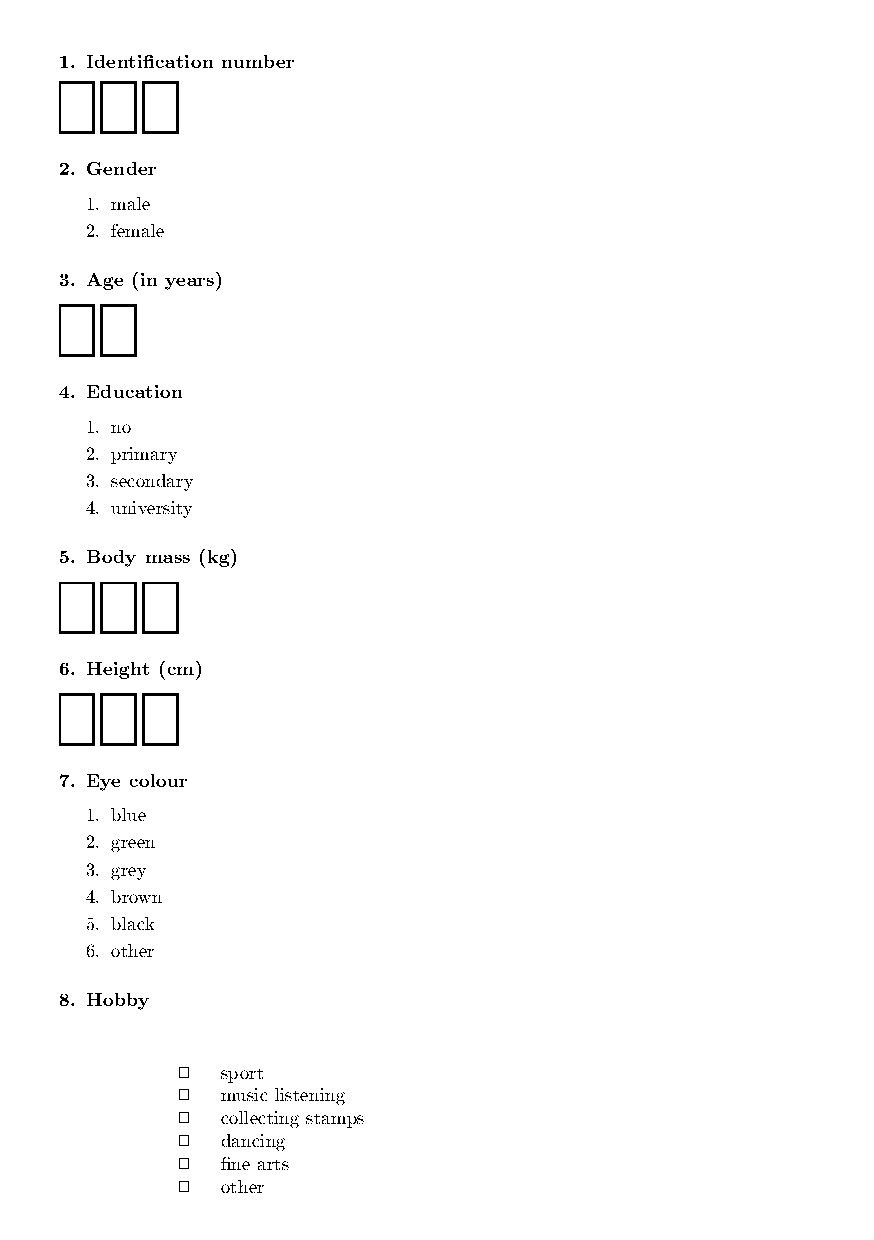
\includegraphics[height=0.8\textheight]{01-kerdoiv.pdf}	\hspace{2em}}
%	\end{center}

\subsection{Create variables using the questionnaire!}

\begin{minipage}{0.48\textwidth}
\centering
	\begin{tabular}{ll}
	\toprule
	variable & type\\
	\midrule
		 ID\\
		 GENDER & categorical, binary\\
		 AGE & \\
		 EDUCATION &categorical, ordinal\\
		 WEIGHT\\
		HEIGHT & continuous, quantitative\\
		  \bottomrule
	\end{tabular}
\end{minipage}
\begin{minipage}{0.48\textwidth}
\centering
	\begin{tabular}{ll}
	\toprule
	variable & type\\
	\midrule
		  E\_COLOUR & categorical, nominal\\
		  SPORT\\
		  MUSIC\\
		  STAMP\\
  		  DANCE&\\
		  FINEART & categorical, binary\\
		  \bottomrule
	\end{tabular}
\end{minipage}



\subsection{Dataset (sample) based on the questionnaire}
\begin{center}
\large
		\begin{tabular}{cccccccccc}
	\toprule
	ID&
	GENDER&
	AGE&
	EDUCATION&
	WEIGHT&
	HEIGHT&
	E\_COLOUR&
	SPORT&
	MUSIC
	\\
	\midrule
	1&1&20&3&65&185&3&1&1\\
	\midrule
	2&2&17&3&60&170&4&1&2\\
	\midrule
	3&1&22&3&62&177&2&2&1\\
	\midrule
	4&2&28&4&62&176&4&2&1\\
	\midrule
	5&1&9&1&32&148&4&2&2\\
	\midrule
	6&1&5&1&19&125&3&2&2\\
	\midrule
	7&2&26&3&70&166&4&2&2\\
	\midrule
	8&1&60&4&75&180&1&1&1\\
	\midrule
	9&2&35&3&49&155&4&2&1\\
	\midrule
	10&2&51&4&61&162&4&2&1\\
	\midrule
	11&1&17&2&61&178&4&2&1\\
	\midrule
	12&2&50&2&65&164&4&2&2\\
	\midrule
	13&1&9&1&30&130&2&1&2\\
	\midrule
	14&2&10&1&40&135&1&2&1\\
	\midrule
	15&1&19&3&86&187&3&1&1\\
	\midrule
	16&1&22&3&67&179&4&2&2\\
	\midrule
	17&1&25&3&103&186&4&1&1\\
	\midrule
	18&1&29&4&74&176&1&1&1\\
	\midrule
	19&2&27&4&67&164&4&1&1\\
	\midrule
	20&1&19&3&70&180&4&1&1\\
	\bottomrule
	\end{tabular}
\end{center}

\section{Discrete variables: distribution, absolute and relative frequency, bar chart}



\subsection{Characterize the \variable{GENDER} variable.}

\begin{minipage}{0.48\textwidth}
	\emph{Frequency table}
	
	\begin{center}
		\begin{tabular}{l|l|l}
		\toprule
				& frequency	&relative frequency (\%)\\
		\midrule		
		male&&\\
		female&&\\
		\midrule
		Total&&\\
		\bottomrule
		\end{tabular}
	\end{center}
\end{minipage}
\hfill
\begin{minipage}{0.48\textwidth}
	\emph{Bar charts (absolute and relative frequencies)}\smallskip
	
	\begin{tabular}{|llll}
	&&\\\\\\\\\\
	\hline
	\multicolumn{1}{l}{}& male && female
	\end{tabular}
	\quad\quad
		\begin{tabular}{|llll}
		&&\\\\\\\\\\
		\hline
		\multicolumn{1}{l}{}& male && female
		\end{tabular}
\end{minipage}
	
	\clearpage
	\subsection{Characterize the \variable{EDUCATION} variable!}

	\emph{Frequency table}
	
	\begin{center}
		\begin{tabular}{l|l|l}
		\toprule
				& frequency	& relative frequency (\%)\\
		\midrule		
		No&&\\
		Primary school&&\\
		Secondary school &&\\
	   University&&\\
		\midrule
		Total&&\\
		\bottomrule
		\end{tabular}
	\end{center}

	\noindent\emph{Bar chart -- (absolute) frequency}\smallskip
		
	\begin{center}
		\begin{tabular}{|llllllllllll}
		&&\\\\\\\\\\
		\hline
		\multicolumn{1}{l}{}& no && primary && secondary && university
		\end{tabular}
	\end{center}
	
		\noindent\emph{Bar chart -- relative frequency}\smallskip
			
		\begin{center}
			\begin{tabular}{|llllllllllll}
			&&\\\\\\\\\\
			\hline
			\multicolumn{1}{l}{}& no && primary && secondary && university
			\end{tabular}
		\end{center}
		
	

%\chapter[Distribution of continuous variables]{Distribution of\\ continuous variables}

%\begin{center}	\begin{tabular}{cccccccccc}
	\toprule
	ID&
	GENDER&
	AGE&
	EDUCATION&
	WEIGHT&
	HEIGHT&
	E\_COLOUR&
	SPORT&
	MUSIC
	\\
	\midrule
	1&1&20&3&65&185&3&1&1\\
	\midrule
	2&2&17&3&60&170&4&1&2\\
	\midrule
	3&1&22&3&62&177&2&2&1\\
	\midrule
	4&2&28&4&62&176&4&2&1\\
	\midrule
	5&1&9&1&32&148&4&2&2\\
	\midrule
	6&1&5&1&19&125&3&2&2\\
	\midrule
	7&2&26&3&70&166&4&2&2\\
	\midrule
	8&1&60&4&75&180&1&1&1\\
	\midrule
	9&2&35&3&49&155&4&2&1\\
	\midrule
	10&2&51&4&61&162&4&2&1\\
	\midrule
	11&1&17&2&61&178&4&2&1\\
	\midrule
	12&2&50&2&65&164&4&2&2\\
	\midrule
	13&1&9&1&30&130&2&1&2\\
	\midrule
	14&2&10&1&40&135&1&2&1\\
	\midrule
	15&1&19&3&86&187&3&1&1\\
	\midrule
	16&1&22&3&67&179&4&2&2\\
	\midrule
	17&1&25&3&103&186&4&1&1\\
	\midrule
	18&1&29&4&74&176&1&1&1\\
	\midrule
	19&2&27&4&67&164&4&1&1\\
	\midrule
	20&1&19&3&70&180&4&1&1\\
	\bottomrule
	\end{tabular}\end{center}

\section{Continuous variables: absolute and relative frequency, histogram}
\subsection{Characterize the \variable{AGE} variable! Create a histogram, make scale on $y$-axis.\\ Interpret the results!}




	\noindent\emph{Frequency table}\hfill\emph{Frequency and relative frequency histogram}
	
	\begin{center}
		\begin{tabular}{l|l|l}
		\toprule
		AGE		& frequency	& relative frequency (\%)\\
		\midrule		
	$\left[0,10\right)$&&\\
	$\left[10,20\right)$&&\\
	$\left[20,30\right)$&&\\
	$\left[30,40\right)$&&\\
	$\left[40,50\right)$&&\\
	$\left[50,60\right)$&&\\
	$\left[60,70\right)$&&\\
		\midrule
		total&&\\
		\bottomrule
		\end{tabular}
%	\end{center}
%
%\noindent
%	\begin{center}
\hfill
\footnotesize
	\begin{tabular}{|llllllll}
		&&\\\\\\\\\\\\\\
		\hline
		\multicolumn{1}{l}{}& 10 & 20 & 30 & 40 & 50 & 60 & 70
\\
\\
\\
		&&\\\\\\\\\\\\\\
		\hline
		\multicolumn{1}{l}{}& 10 & 20 & 30 & 40 & 50 & 60 & 70
		\end{tabular}
	\end{center}

%\subsubsection*{Interpret the results!}
\begin{enumerate}
\item Is the shape of the distribution symmetrical (or skewed)?
\item Which interval contains the most/fewest elements?
\end{enumerate}

\subsubsection*{Double the interval width. Create histograms using data of variable \variable{AGE}. Make scale on $y$-axis.}


%	\emph{Gyakoriság táblázat}
	
	\begin{center}\small
		\begin{tabular}{l|l|l}
		\toprule
		AGE		& frequency	& relative frequency (\%)\\
		\midrule		
	$\left[0,20\right)$&&\\
	$\left[20,40\right)$&&\\
	$\left[40,60\right)$&&\\
	$\left[60,80\right)$&&\\		
		\midrule
		total&&\\
		\bottomrule
		\end{tabular}		
		\hfill\footnotesize
		\begin{tabular}{|llllllll}
		&&\\\\\\\\\\\\\\
		\hline
		\multicolumn{1}{l}{}& 20 && 40 && 60 && 80
		\end{tabular}
		\hfill
		\begin{tabular}{|llllllll}
		&&\\\\\\\\\\\\\\
		\hline
		\multicolumn{1}{l}{}& 20 && 40 && 60 && 80
		\end{tabular}
	\end{center}


\subsection{Characterize the \variable{WEIGHT} variable as done it for variable \variable{AGE}!}

	\begin{center}\small
		\begin{tabular}{l|l|l}
		\toprule
		WEIGHT		& frequency	& relative frequency (\%)\\
		\midrule		
	$\left[0,20\right)$&&\\
	$\left[20,40\right)$&&\\
	$\left[40,60\right)$&&\\
	$\left[60,80\right)$&&\\
	$\left[80,100\right)$&&\\
	$\left[100,120\right)$&&\\										
		\midrule
		total&&\\
		\bottomrule
		\end{tabular}		
		\hfill\footnotesize
		\begin{tabular}{|llllllllllll}
		&&\\\\\\\\\\\\\\
		\hline
		\multicolumn{1}{l}{}& 20 && 40 && 60 && 80 && 100&& 120
		\end{tabular}
	\end{center}
\section{Continuous variables: measures of central tendency and variability}
\subsection{Calculate mean, median, mode, range, standard deviation of these random samples.}\label{subsec:descriptive}

\begin{center}\large
	\begin{tabular}{c|c|c|c|c|c||c|c}
	\toprule
		&$n$&Random sample&
		Mean&
		Median&
		Mode&
		Range&
		Standard deviation\\		
	\midrule
		1.&$n = 4$&1 2 4 1&&&&&\\
		2.&$n = 4$&10 20 40 10&&&&&\\
		3.&$n = 4$&2 4 8 2&&&&&\\
		4.&$n = 4$&2 3 5 2&&&&&\\
		5.&$n = 6$&1 3 2 4 0 2&&&&&\\
	\bottomrule
	\end{tabular}
\end{center}



%\subsubsection*{Compare the mean and the median. Conclude to the symmetry of the distribution.}

\subsection{The numbers of some special operations made by 15 man operators are the following}


	\begin{center}
		20  25  25  27  28  31  33  34  36  37  44  50  59  85  86
	\end{center}	

%The histogram of the sample can be seen below:
	  
	
	\subsubsection*{Based on the shape of the histogram, which statement is true? Why?}
	\begin{wrapfigure}{R}{0.4\textwidth} \vspace{-100pt}
	  \begin{flushright}
	  	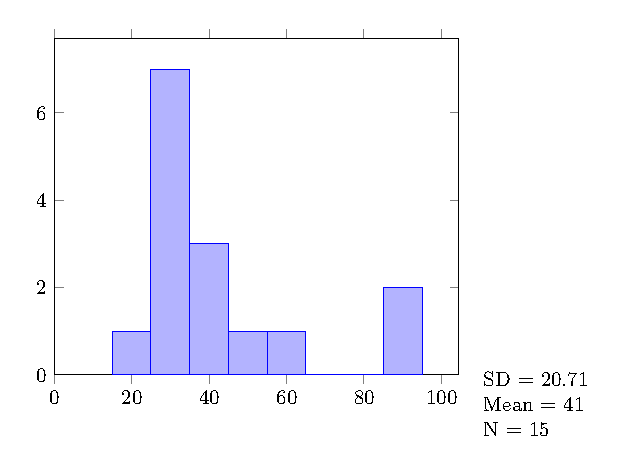
\includegraphics[width=0.36\textwidth]{02-ferfi-operalas}
	  	\vspace{-140pt}
	  \end{flushright}
	\end{wrapfigure}	
	\begin{enumerate}
	\item the mean is smaller than the median
	\item the mean is approximately equal to the median
	\item the mean is greater than the median
	\end{enumerate}

	\subsubsection*{Find the quartiles of the above sample.}
	\begin{enumerate}
	\item first (lower) quartile (25\% percentile):
	\item second quartile (50\% percentile, median):
	\item third (upper) quartile (75\% percentile):
	\end{enumerate}

	\clearpage
	\subsubsection*{Draw a box plot. Compare this to the histogram.\\
		Draw a mean-SD diagram. Can you conclude to the symmetry of the distribution based on this diagram?}
	\vspace{10em}

\subsection{The numbers of some special operations made by 10 woman operators are the following:}


	\begin{center}
	5  7  10  14  18  19  25  29  31  33
	\end{center}	
  	
	\subsubsection*{Based on the shape of the histogram, which statement is true? Why?}
	%The histogram of the sample can be seen below:
	\begin{wrapfigure}{R}{0.4\textwidth} \vspace{-140pt}
	  \begin{flushright}
	  	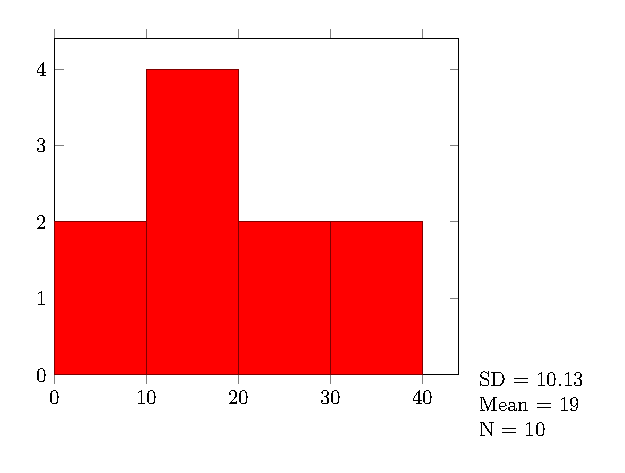
\includegraphics[width=0.36\textwidth]{02-no-operalas}
	  \vspace{-140pt}
	  \end{flushright}
	\end{wrapfigure}	
	

	\begin{enumerate}
	\item the mean is smaller than the median
	\item the mean is approximately equal to the median
	\item the mean is greater than the median
	\end{enumerate}

	\subsubsection*{Find the quartiles of the above sample.}
	\begin{enumerate}
	\item first (lower) quartile (25\% percentile):
	\item second quartile (50\% percentile, median):
	\item third (upper) quartile (75\% percentile):
	\end{enumerate}



	\subsubsection*{Draw a box plot. Compare this to the histogram.\\
	Draw a mean-SD diagram. Can you conclude to the symmetry of the distribution based on this diagram?}
	\vspace{10em}

%\clearpage
\subsection[Putting the diagrams side by side, the two distributions can be compared.]{Putting the diagrams side by side, the two distributions can be compared.\\ Which diagram gives more information and why?}

	\begin{center}
	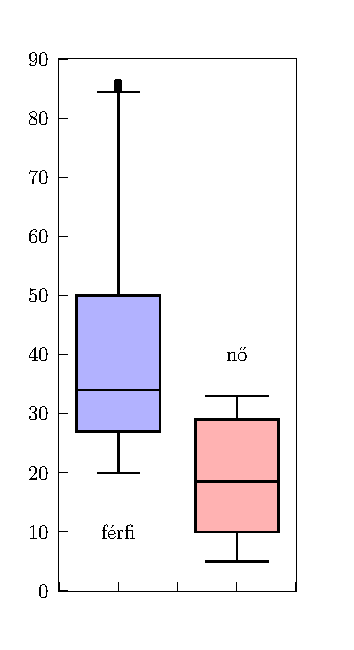
\includegraphics[width=0.15\textwidth]{02-boxplot}
	\hspace{4em}
	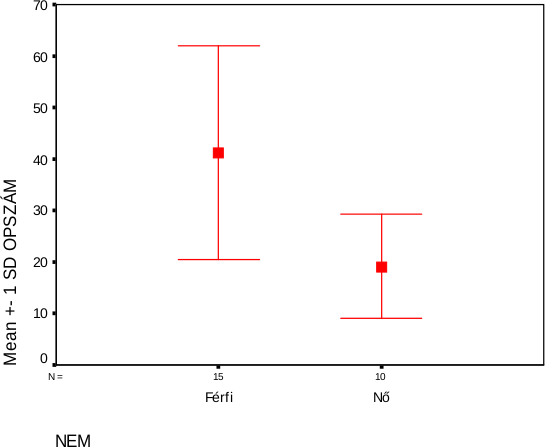
\includegraphics[width=0.2\textwidth]{02-sd}
	\end{center}
	
\section{Calculations with R}

\subsection{Type the samples from the Exercise \ref{subsec:descriptive} in  R and calculate the descriptive statistics.}


\subsection{Open the \data{smallquest\_labels.csv} data file!	
	Repeat the characterization of both \variable{GENDER}, \variable{EDUCATION}, \variable{AGE} and \variable{WEIGHT} variables using the R commands}
	

\subsection{Open the \data{bank.csv} data file. Characterize the continuous variables. Calculate the descriptive statistics of all the continuous variables, e.g. \variable{salnow} (current salary). Interpret the results.}


%\begin{center}	
%	\begin{tabular}{c|c|c|c|c|c|c||c}
%	\toprule
%Variable&
%Min&
%Max&
%Range&
%Mean&
%Median&
%Mode&
%SD\\
%	\midrule
%	&&&&&&&\\
%	&&&&&&&\\
%	&&&&&&&\\		
%	\bottomrule
%	\end{tabular}
%\end{center}


\section{Homework}
\subsection{Here are the blood types of 20 patients. Characterize the distribution of this data.}
	\begin{center}A  0  0  B  AB  0  A  B  B  AB  0  A  0  AB  B  0  AB  0  B  AB\end{center}

\subsection{Given the following temperature values. Calculate summary statistics for the sample, construct a frequency histogram and a box diagram. Conclude to the symmetry of the distribution.}
	\begin{center}35.1  36.1  35.2  36.2  36.5  36.5  37  36.2  36.8  36.7  36.5\end{center}

	
\subsection{Consider the following ordered set of data. Find the mean, first quartile, median, third quartile, range, mode, standard deviation of this data.}
	\begin{center}44  49  50  51  53  57  58  62  66  66  68  71  75  77  80  85\end{center}

	
\subsection{Interpret the results of the table below (Varga Z et al: Individualized positioning for maximum heart protection breast irradion. Acta Oncologica 2013)}

	\begin{center}
	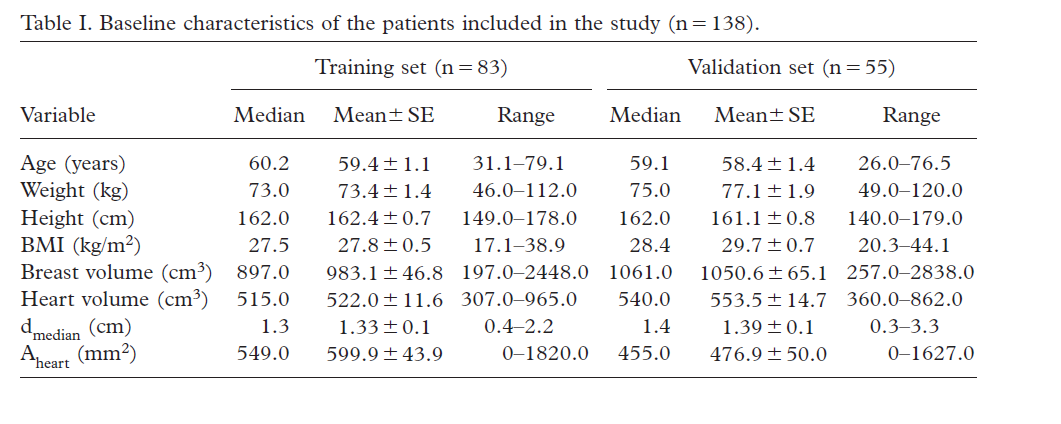
\includegraphics[width=0.7\textwidth]{Adat/02-continuous-table}
	\end{center}

	\chapter[Probability and distributions]{Probability, conditional probability, diagnostic tests, discrete and normal distributions}
%VALÓSZÍNŰSÉG, FELTÉTELES VALÓSZÍNŰSÉG, DIAGNOSZTIKUS TESZTEK, DISZKRÉT ELOSZLÁSOK, NORMÁLIS ELOSZLÁS
\renewcommand{\P}{\mathrm{P}}
\section{Probability calculus}

\subsection{If we roll a dice, there are 6 possible outcomes.}
If $X$ represents the value of the outcome, find the following probabilities: 
\begin{enumerate}[a)] 
\item $\P(X = 1)=$ \hrulefill
\item $\P(X > 1)=$ \hrulefill
\item $\P(1 < X < 4)=$ \hrulefill
\end{enumerate}


\subsection{If we roll two dices, there are 36 possible outcomes.}
	\textbf{If $X$ represents the sum, $Y$ the product of the rolled numbers, find the following probabilities:}
	
	\begin{multicols}{2}	
		\begin{enumerate}[a)] 
		\item $\P(X = 2)=$ \hrulefill
		\item $\P(X > 2)=$ \hrulefill
		\item $\P(X = 10)=$ \hrulefill
		\item $\P(Y = 2)=$ \hrulefill
		\item $\P(Y = 12)=$ \hrulefill
		\end{enumerate}
		
	\columnbreak
		
	\begin{flushright}
		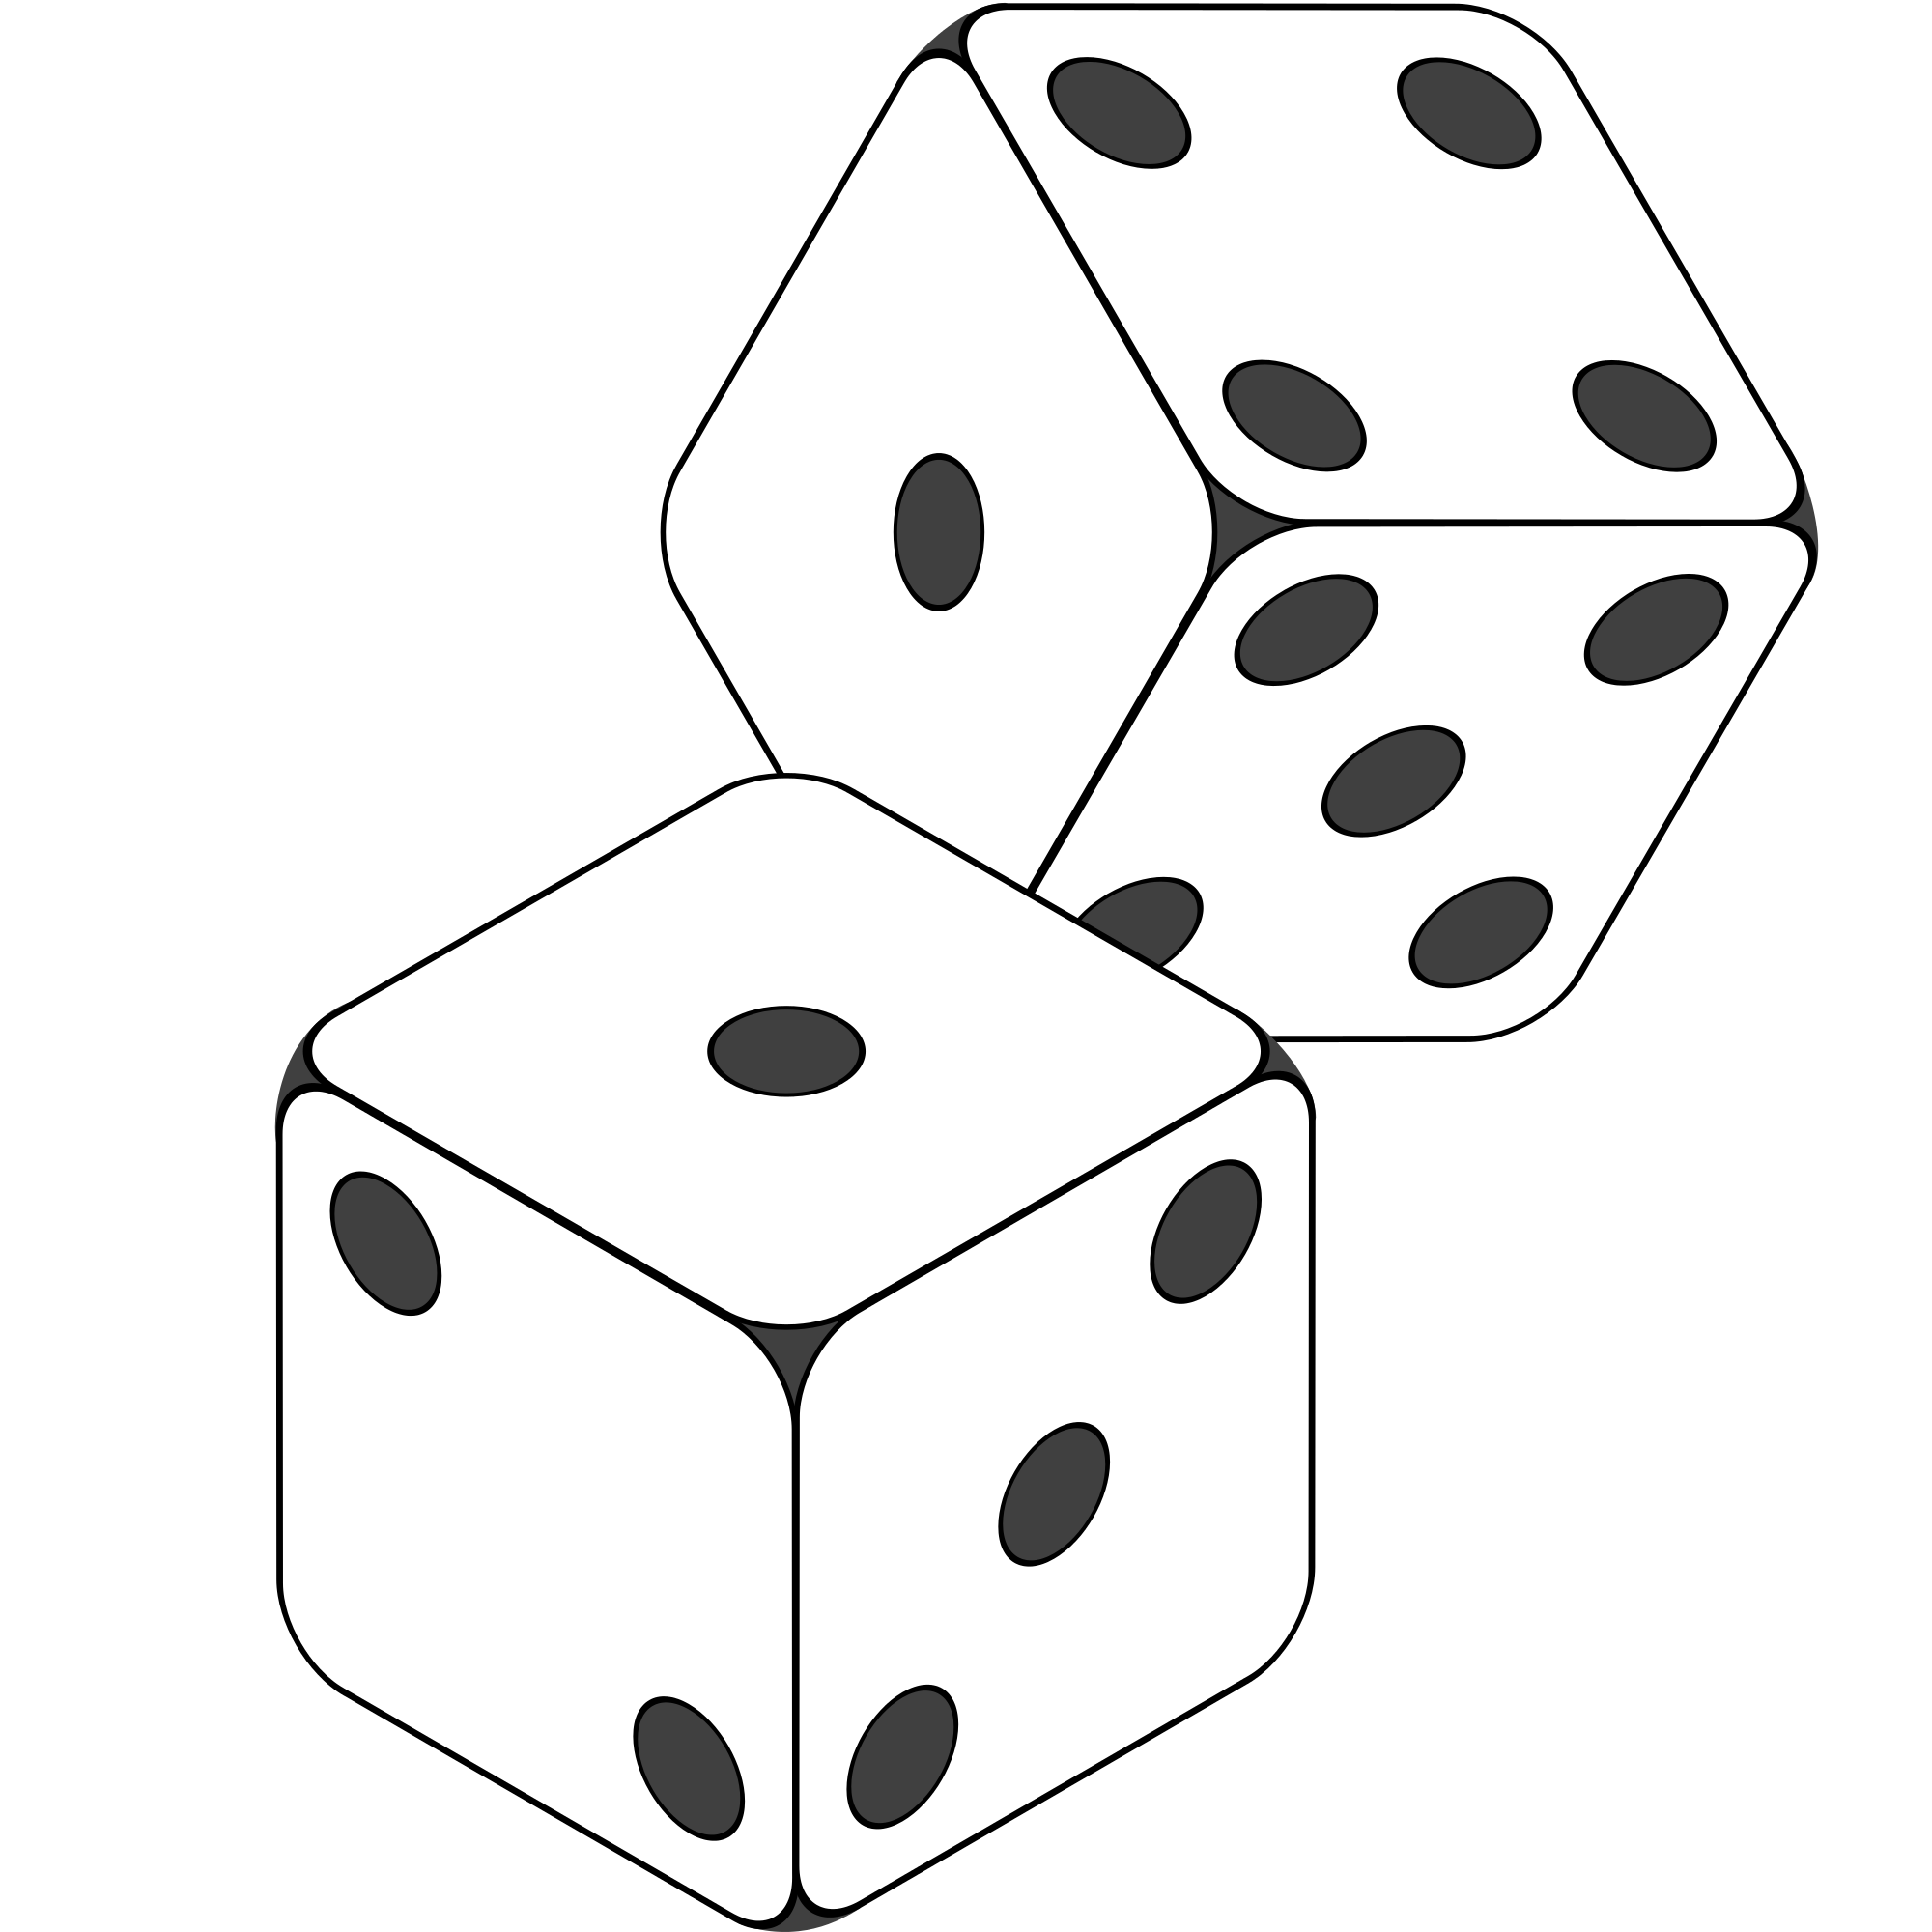
\includegraphics[width=10em]{Dice}
	\end{flushright}
	\end{multicols}	

\subsection{A fair coin is tossed twice.}


\begin{enumerate}[a)] 
\item List the possible outcomes: \hrulefill
\item Find the probability of getting two heads: \hrulefill
\end{enumerate}

\vspace{-8em}
\begin{flushright}
	\includegraphics[width=14em]{head-tail}%English_Two_Shillings_1938.jpg}
	
	head \hspace{5em} tail\hspace*{2.5em}
\end{flushright}


\subsection{A penny is tossed once and a dice is rolled once}

\begin{enumerate}[a)] 
\item List the possible outcomes: 	 \hrulefill

\textbf{Find the probabilities of the following outcomes:}
\item tossing a head and rolling an even number: \hrulefill
\item tossing a head or rolling an even number: \hrulefill
\item tossing a head and rolling a 5: \hrulefill	
\item tossing a head or rolling a 5: \hrulefill 	
\item rolling either a 4 or a 6: \hrulefill	
\end{enumerate}


%TODO ez nincs benne a magyarban
\subsection{The blood groups of 200 people are distributed as follows}
50 have blood type A, 65 have blood type B, 70 have blood type 0 and 15 have blood type AB. If a person from this group is selected at random, what is the probability that this person has blood type 0?


\section{Discrete distributions}
\subsection{A penny is tossed 3 times}
Elementary events: \hrulefill
\\
Define the variable $X$ to be the number of heads. Prepare the distribution of the variable $X$.



\newcolumntype{L}[1]{>{\raggedright\let\newline\\\arraybackslash\hspace{0pt}}m{#1}}
\newcolumntype{C}[1]{>{\centering\let\newline\\\arraybackslash\hspace{0pt}}m{#1}}
\newcolumntype{R}[1]{>{\raggedleft\let\newline\\\arraybackslash\hspace{0pt}}m{#1}}


\begin{center} 
%{\renewcommand{\arraystretch}{1.5} %<- modify value to suit your needs
	\begin{tabular}{c|C{1cm}|C{1cm}|C{1cm}|C{1cm}}
	\toprule
	$X$		& 0 & 1 & 2 & 3\\
	\midrule
	$\P(X)$ &&&&\\
	\bottomrule
	\end{tabular}
\end{center}


\subsection{Which of the following distributions are probability distributions?}
\begin{enumerate}[a)]
\item 

	\begin{tabular}{c|C{1cm}|C{1cm}|C{1cm}|C{1cm}|C{1cm}}
	\toprule
	$X$		& 0 & 5 & 10 & 15 & 20\\
	\midrule
	$\P(X)$ &1/5 &1/5&	1/5&	1/5&	1/5\\
	\bottomrule
	\end{tabular}


\item 

	\begin{tabular}{c|C{1cm}|C{1cm}|C{1cm}|C{1cm}}
	\toprule
	$X$		&0 & 2 & 	4 &	6 	\\
	\midrule
	$\P(X)$ &1/4&	1/8&	1/16&	9/16	\\
	\bottomrule
	\end{tabular}

\item 

	\begin{tabular}{c|C{1cm}|C{1cm}|C{1cm}|C{1cm}}
	\toprule
	$X$		&0 & 2 & 	4 &	6
	\\
	\midrule
	$\P(X)$ &-1& 1.5 &	0.30 & 0.2	\\
	\bottomrule
	\end{tabular}

\item	
	\begin{tabular}{c|C{1cm}|C{1cm}|C{1cm}|C{1cm}}
	\toprule
	$X$		&0 & 2 & 	4 &	6 	\\
	\midrule
	$\P(X)$ &1/4&	1/8&	1/16&	2/16	\\
	\bottomrule
	\end{tabular}	
\end{enumerate}


\section{Conditional probability}
\subsection[Conditional probability of having girls and boys]{We have large number of families with two children.  After selecting randomly a girl from this set of families estimate the probability of the event that there is a boy also in that family.}

 	
\begin{enumerate}[a)]
\item List of the elementary events: \hrulefill
\item Event $A$: \emph{there is at least one girl in the family}\quad GB, BG, GG
	\qquad
	$\P(A) =$ 	\hrulefill
\item Event $B$: \emph{there is at least one boy in the family}\quad \hrulefill
	\qquad
	$\P(B) =$ 	\hrulefill
\item Event $A$ and $B$ ($A\cdot B$): \hrulefill
	
	Possible cases from the list of elementary events: \hrulefill	
	
	$\P(AB) =$ 	\hrulefill


\item Conditional probability is $\P(B|A)= \frac{\P(AB)}{\P(A)} =$ \hrulefill	
\end{enumerate}


\subsection[Probability of 2 being rolled if the reult is even]{Calculate the probability of a 2 being rolled by a dice if it is already known that the result is even}

\noindent\hrulefill
\subsection{A dice is rolled twice, we got different numbers.}
What is the probability that at least one of them is a 6?



\noindent\hrulefill


\section{Diagnostic tests}
\subsection{Relation between results of liver scan and correct diagnosis are summarised in the following table.}
 Calculate sensitivity, specificity, positive (PPV) and negative (NPV) predictive values.

\hfill Source: D G Altman, J M Bland BMJ 1994; 308:1552


\begin{center}
	\begin{tabular}{r|cc|l}
	\toprule
			& \multicolumn{2}{c|}{\textbf{Pathology}}\\
	\textbf{Liver scan}	& abnormal (+)	& normal (-)	&Total\\
	\midrule
	abnormal (+) &	231	&32	&263\\
	normal (-)&	27	&54	&81\\
	\midrule
	Total		&258&	86	&344\\
	\bottomrule	
	\end{tabular}
\end{center}

\begin{enumerate}[a)]
\item Sensitivity: \hrulefill
\item Specificity: \hrulefill
\item PPV:	\hrulefill
\item NPV:	\hrulefill
\item Proportion of all correct diagnosis: \hrulefill
\item What does sensitivity mean? 	\hrulefill
\item What is the probability of abnormal pathology test result given abnormal liver scan result? \hrulefill
\end{enumerate}



\subsection{In the following table, the observed frequencies of two diagnostic tests are summarised. Calculate sensitivity, specificity, positive and negative predictive values.}


\begin{center}
	\begin{tabular}{r|cc|l}
	\toprule
			& \multicolumn{2}{c|}{\textbf{standard test}}\\
	\textbf{new test	}	& +	& -	&Total\\
	\midrule
	+ & 60 & 35\\
	- &	40 & 65\\
	\midrule
	Total	&&	&\\
	\bottomrule	
	\end{tabular}
\end{center}


\begin{enumerate}[a)]
\item Sensitivity: \hrulefill
\item Specificity:	\hrulefill
\item PPV:	\hrulefill
\item NPV:	\hrulefill
\item Proportion of all correct diagnosis: \hrulefill
\item What does positive predictive value (PPV) mean? 	\hrulefill
\item What is the probability of negative new test result in case of negative standard test result? \hrulefill
\end{enumerate}



\clearpage
\section{Normal distributions}

\newcommand{\N}{\mathcal{N}}
\subsection{Draw the $\N(1, 1), \N(2, 1), \N(-1, 1)$ normal distributions, if the curve of the $\N(0, 1)$ distribution is given:}

\begin{center}
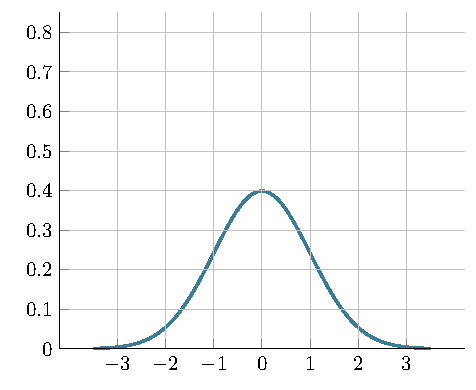
\includegraphics[height=0.37\textwidth]{03-standard-normalis}
\end{center}


\subsection{Draw the $\N(0, 2^2), \N(0, 0.5^2)$ normal distributions, if the curve of the $\N(0, 1)$ distribution is given!} 

\begin{center}
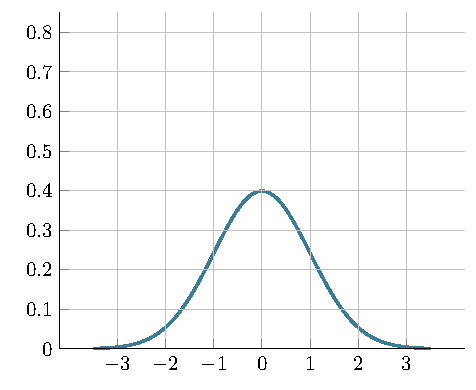
\includegraphics[height=0.37\textwidth]{03-standard-normalis}
\end{center}

\subsection{Draw the $\N(2, 2^2), \N(1, 2^2)$ normal distributions, if the curve $\N(3, 2^2)$ is given!}
\begin{center}
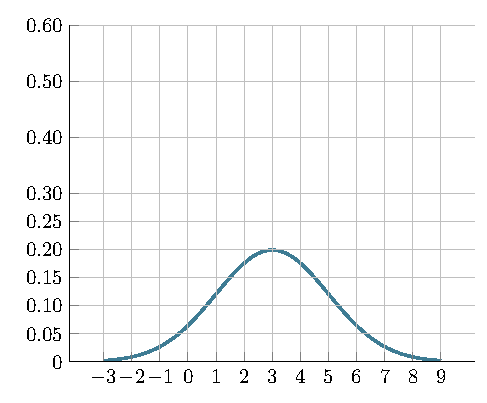
\includegraphics[height=0.37\textwidth]{03-standard-normalis2}
\end{center}



\subsection{For a standard normal distribution, find the following probabilities:}


\begin{enumerate}[a)]
\item $\P(Z < 0) =$ %Mi a valószínűsége, hogy a változó értéke 0-nál kisebb? 
	\hrulefill
\item $\P(Z > 0) =$ %Mi a valószínűsége, hogy a változó értéke 0-nál kisebb? 
	\hrulefill
\item $\P(Z < -1) =$ %Mi a valószínűsége, hogy a változó értéke -1-nél kisebb? \hrulefill	
	\hrulefill
\item $\P(Z > 1) =$ % Mi a valószínűsége, hogy a változó értéke 1-nél nagyobb?	\hrulefill
	\hrulefill
\item $\P(Z < -1,96) = 	$ \hrulefill
\item $\P(-1 < Z < 1) =$ \hrulefill
\item $\P(-1,96 < Z < 1,96) =$ \hrulefill
\item $\P(-2 < Z < 2) = $ \hrulefill
\item Find $x$ value such that the area to the left of $x$ is 0.025: \hrulefill
\item Find $x$ value such that the area to the left of $x$ is 0.5: \hrulefill
\item Which interval contains the middle 95\% of the data? \hrulefill
\item Which interval contains the middle 99\% of the data? \hrulefill
\end{enumerate}


\begin{table}[!h]\centering \small
\caption{Standard normal distribution}


 
	$\Phi(x)=\P(Z < x) =$ proportion of area to the left of $x$ (gray area)

	\begin{minipage}{0.4\textwidth}\flushright
		\begin{tabular}{ll}
		\toprule
		$x$		& $\Phi(x)$ \\
		\midrule
		$-\infty$	& $0$\footnote{limit}\\
		-4.5		& 0.00001\\
		-4		& 0.00003\\
		-3.5		& 0.00023\\
		-3		& 0.00135\\
		\midrule
		-2.576		& 0.005\\
		-2.5		& 0.00621\\
		-2.326		& 0.01\\
		-2		& 0.02275\\
		\midrule
		-1.96		& 0.025\\
		-1.645		& 0.05\\
		-1.5		& 0.06681\\
		-1		& 0.15865\\
		\midrule		
		-0.5		& 0.30854\\
		0		& 0.5\\
		0.5		& 0.69146\\
		\midrule
		1		& 0.84135\\
		1.5		& 0.93319\\
		1.645		& 0.95\\
		1.96		& 0.975\\		
		\bottomrule
		\end{tabular}\hspace{2em}
	\end{minipage}
	\begin{minipage}{0.4\textwidth}
		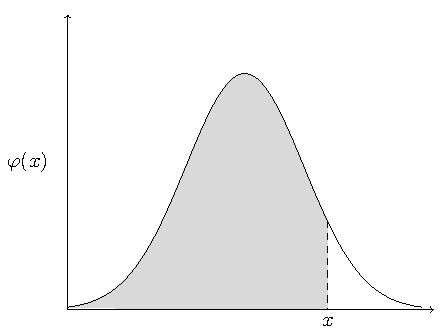
\includegraphics[width=0.95\textwidth]{03-standard-normalis-szurkitett}

		\begin{tabular}{ll}
		\toprule
		$x$		& $\Phi(x)$ \\
		\midrule
		2		& 0.97725\\
		2.326		& 0.99\\
		2.5		& 0.99379\\
		2.576		& 0.995\\
		\midrule
		3		& 0.99865\\
		3.5		& 0.99977\\
		4		& 0.99997\\
		4.5		& 0.99999\\
		$\infty$	& $1^a$\\
		\bottomrule
		\end{tabular}
		\end{minipage}		
\end{table}



\subsection{The results in a certain blood test performed in a medical laboratory are known to be normally distributed with $\N(60, 10^2)$}



\begin{enumerate}[a)]
\item What percentage of the results are below 60? 		 \hrulefill

	What percentage of the results are above 60? \hrulefill
\item What percentage of the results are between 40 and 80? 	 	 \hrulefill

What percentage of the results are below 40? 	 \hrulefill

What percentage of the results are above 80? 	 \hrulefill

\item The ''healthy range'' falls between 30 and 90. 

	What percentage of the results are between 30 and 90? \hrulefill

	What percentage of the results are outside the healthy range of 30 to 90? 	 \hrulefill
\end{enumerate}

\subsection {At an urban hospital the weights of new-born infants are normally distributed with $\N(3500, 400^2)$. Let X be the weight of a new-born picked at random. Find the following probabilities:}



\begin{enumerate}[a)]
\item $\P(X < 3500):$ \hrulefill 	
\item $\P(3100 < X < 3900):$ \hrulefill	
\item Determine the middle interval where 95\% of the weights will fall.

	 \hrulefill
\end{enumerate}


\section{Homework}

\subsection{After performing a diagnostic test we have the following frequencies:}

\begin{center}\small
	\begin{tabular}{r|cc|l}
	\toprule
			& \multicolumn{2}{c|}{\textbf{standard test}}\\
	\textbf{new test}	& +	& -	&Total\\
	\midrule
	+ & 60 & 20 & 80\\
	- &	40 & 80 & 120\\
	\midrule
	Total	&100&100	&200\\
	\bottomrule	
	\end{tabular}
\end{center}

Determine the asked proportions and give the name of the measure!
\begin{enumerate}[a)]
\item What is the proportion of people who test positive (new test +) for the disease among those who have the disease (standard test +)?\hrulefill%sensitivity


\item What is the proportion of people who test negative (new test -) for the disease among those who don't have the disease (standard test -)?
 \hrulefill% specificity


\item The proportion of the true positives among those who had positive results based on the new test?
%Az összes, az új teszt által betegnek (pozitívnak) minősített esetből mennyi a valóban betegek (valódi pozitívok) aránya?

 \hrulefill


\item The proportion of the true negatives among those who had negative results based on the new test?

\hrulefill
%Az összes, az új teszt által egészségesnek (negatívnak) minősített esetből mennyi a valóban egészséges (valódi negatívok) aránya?


\end{enumerate}

\subsection{A normal distribution has a mean of 30 and a standard deviation of 10. 
What proportion of the distribution is above 50?}
\vspace{5em}

\subsection{A ball is drawn from a box containing 10 blue balls, 10 black and 5 green. What is the probability that the ball will be green given that it is not black?}
\vfill

	\chapter[Confidence intervals]{Confidence\\ intervals}
\section[Confidence interval for the population mean if the population SD is known]{
Confidence interval for the population mean ($\mu$) if the population standard deviation ($\sigma$) is known}

\subsection{Assume that the heights of first year pharmaceutical students are normally distributed with a mean of $\mu = 175$ and a standard deviation of $\sigma=10$.}

\begin{enumerate}[a)]
\item What percentage of heights are above 175 cm? 	\hrulefill
\item What percentage of heights are below 175 cm? 	\hrulefill
\item What percentage of heights are between 155 and 195? 	\hrulefill
\item What percentage of heights are below 155 cm? 	 \hrulefill
\item Calculate the mean and the standard error of the mean of a sample of 36 cases derived from this population.

	\begin{enumerate}[i)]
	\item mean? \hrulefill
	\item standard error? \hrulefill
	\end{enumerate}

\item The mean of another random sample with 36 number of cases is 172. 
	\begin{enumerate}[i)]
	\item Calculate the 95\% confidence interval.  \hrulefill
	\item What is the meaning of the 95\% CI? \hrulefill
	\item Compare the population mean with the 95\% CI calculated. 
		Is the population mean included in the 95\% CI? \hrulefill
	\end{enumerate}
\end{enumerate}


\section[Confidence interval for the population mean if the population SD is unknown]{
Confidence interval for the population mean ($\mu$)
if the population standard deviation ($\sigma$) is unknown
}
	
	
\subsection{(Example from Altman). In a trial we actually observed a mean serum albumin of 34.46 g/l with a standard deviation of 5.834 g/l from a sample of 21 patients with primary biliary cirrhosis. }


%SE (standard error): \hrulefill
\begin{enumerate}[a)]
\item Find the 95\% confidence interval.

	\begin{description}
	\item[$\alpha:$] \hrulefill\quad n: 	\hrulefill
	\item[mean:] \hrulefill\quad \textbf{SE:} \hrulefill
	\item[degrees of freedom:]  \hrulefill\quad \textbf{$t_\alpha$:} \hrulefill
	\item[mean - $t_\alpha$ SE:] \hrulefill \quad\quad \textbf{mean + $t_\alpha$ SE:} \hrulefill
	\item[Confidence interval:] \hrulefill
		
		\textit{Meaning:} $\P(\hspace{3em}< \textrm{ true population mean } < \hspace{3em}) = 0.95$

		We can be 95\% confident from this study that the true mean serum albumin among all such patients lies somewhere in the range \rule{15mm}{.4pt} to \rule{15mm}{.4pt} g/l, with 34.46 as our best estimate. This interpretation depends on the assumption that the sample of 21 patients is representative of all patients with the disease.
	\end{description}

\clearpage
\item Find the 99\% confidence interval and compare to the 95\% CI.
	\begin{description}
	\item[$\alpha:$] \hrulefill\quad n: 	\hrulefill
	\item[mean:] \hrulefill\quad \textbf{SE:} \hrulefill
	\item[degrees of freedom:]  \hrulefill\quad \textbf{$t_\alpha$:} \hrulefill
	\item[mean - $t_\alpha$ SE:] \hrulefill \quad\quad \textbf{mean + $t_\alpha$ SE:} \hrulefill
	\item[Confidence interval:] \hrulefill
		
		Meaning: $\P(\hspace{3em}< \textrm{ true population mean } < \hspace{3em}) = 0.99$
	\end{description}

\item Suppose that the above data were observed from a sample of 210 patients. Find the 95% confidence interval.
	\begin{description}
	\item[$\alpha:$] \hrulefill\quad n: 	\hrulefill
	\item[mean:] \hrulefill\quad \textbf{SE:} \hrulefill
	\item[degrees of freedom:]  \hrulefill\quad \textbf{$t_\alpha$:} \hrulefill
	\item[mean - $t_\alpha$ SE:] \hrulefill \quad\quad \textbf{mean + $t_\alpha$ SE:} \hrulefill
	\item[Confidence interval:] \hrulefill
	\end{description}		
\end{enumerate}

	


	
\subsection{In a study, systolic blood pressure of 10 healthy women was measured}
Calculate the 95\% confidence interval for the population mean,  if the 

\begin{itemize}
 \item  mean was 119, the standard error was 0.664
 
  \hrulefill
 \item  mean was 119, the standard error was 2.1
 
 	\hrulefill
\end{itemize}
Compare the length of this confidence intervals!

\noindent \hrulefill
\subsection{Questions}

	
\begin{enumerate}[a)]
\item Which is wider, a 95\% or a 99\% confidence interval? 	

 \hrulefill
\item   When you construct a 95\% confidence interval, what are you 95\% confident about? 	

	 \hrulefill
\item When computing a confidence interval, when do you use $t$ and when do you use $u$? 	

\hrulefill
\item What does the confidence interval width depend on? 	

\hrulefill
\end{enumerate}

\clearpage

\section{Calculations with R}

\subsection{Calculate the following statistics for \variable{mass} using the \quest!}

\begin{description}
\item[Sample size: ] \hrulefill \quad \textbf{Mean:} \hrulefill
\item[Standard deviation: ] \hrulefill \quad \textbf{Standard error:} \hrulefill
\end{description}

\begin{enumerate}[a)]
\item Assuming that the variable mass follows a normal distribution, determine the 
	\begin{enumerate}[i)]
	\item 95\% confidence interval: \hrulefill
	\item 99\% confidence interval: \hrulefill 	
	\end{enumerate}
\item Can we state that the mean body mass in the population of students is 70? 	

  \hrulefill	

	Explain. \hrulefill
\end{enumerate}


\subsection{Calculate the following statistics for \variable{height} using the \quest!}

\begin{description}
\item[Sample size: ] \hrulefill \quad \textbf{Mean:} \hrulefill
\item[Standard deviation: ] \hrulefill \quad \textbf{Standard error:} \hrulefill
\end{description}

\begin{enumerate}[a)]
\item Assuming that the variable height follows a normal distribution, determine the 
	\begin{enumerate}[i)]
	\item 95\% confidence interval: \hrulefill
	\item 99\% confidence interval: \hrulefill 	
	\end{enumerate}
\item Can we state that the mean height in the population of students is 170? 	

  \hrulefill	

	Explain. \hrulefill
\end{enumerate}

\section{Homework}

\subsection{A researcher set a 95\% confidence interval on the mean length of fish in a recreational lake and found it to be from 6.2 to 8.7 inches.} 
\textbf{Which of the following is a proper interpretation of this interval?}

\begin{enumerate}[(A)]
\item Of the fish in the recreational lake, 95\% are between 6.2 and 8.7 inches long.
\item We are 95\% confident that the sample mean length of fish in the recreational lake is between 6.2 and 8.7 inches.
\item We are 95\% confident that the population mean length of fish in the recreational lake is between 6.2 and 8.7 inches.
\item There is a 95\% chance that a randomly selected fish from the recreational lake will be between 6.2 and 8.7 inches.
\end{enumerate}

\subsection{An industrial designer wants to determine the average amount of time it takes an adult to assemble an ''easy to assemble'' toy. A sample of 16 times yielded an average time of 19.92 minutes, with a sample standard deviation of 5.73 minutes. Assuming normality of assembly times, provide a 95\% confidence interval for the mean assembly time.}
	

	\chapter[One-sample, two-sample and paired $t$-tests]{One-sample, two-sample\\ and paired $t$-tests}
\section{One-sample $t$-test for the mean of a normal population}
\subsection{The following are the systolic blood pressures (mm Hg) of $n = 9$ patients undergoing drug therapy for hypertension:}

\begin{center}
182.00  152.00  178.00  157.00  194.00  163.00  144.00  114.00  174.00
\end{center}


\textbf{The mean = 162 mm Hg, the standard deviation SD = 23.92.}


\begin{enumerate}[a)]
\item Find the standard error.	\hrulefill
\item Find the 95\% confidence interval for the population mean.	
	 \hrulefill

	What is the meaning of this interval? 	  \hrulefill	

\item \textbf{We would like to test whether the sample is drawn from a population where $\mu = 130$.}

Find the null- and alternative hypothesis.
	
	H$_0$:	\hrulefill
	
	H$_A$:	\hrulefill
	
	\begin{description} %[i)]
	\item[Based on the confidence interval]
	Can we conclude with 95\% confidence on the basis of these data that the population mean is different from 130? 
	Explain your decision. 
	
	\hrulefill
	
	\item[Based on the $t$ test-statistics]
	


	Is the population mean significantly different from 130 at 5\% level?
	
	$t = \frac{\textrm{mean} - 130}{SE} =$ 	\hrulefill
	
Compare its absolute value to the t-value of the table. 	 \hrulefill
		
		Explain your decision. 	\hrulefill
	\item[Based on the $p$-value]
	The $p$-value given by R is $p = 0.004$.
	
	Is there a significant difference from the hypothesized population mean 130 at 5\% level?

		\hrulefill

	\end{description}
\item \textbf{We would like to test whether the sample is drawn from a population where $\mu = 150$.}
	
Find the null- and alternative hypothesis.
		
		H$_0$:	\hrulefill
		
		H$_A$:	\hrulefill
		
		\begin{description}
		\item[Based on the confidence interval]
	Can we conclude with 95\% confidence on the basis of these data that the population mean is different from 150? 
	Explain your decision. 
	
	\hrulefill
	
	\item[Based on the $t$ test-statistics]
	


	Is the population mean significantly different from 150 at 5\% level?
	
	$t = \frac{\textrm{mean} - 150}{SE} =$ 	\hrulefill
	
Compare its absolute value to the t-value of the table. 	 \hrulefill
		
		Explain your decision. 	\hrulefill
	\item[Based on the $p$-value]
			The $p$-value given by R is $p = 0.171$.
	
			Is there a significant difference from the hypothesized population mean 150 at 5\% level?
		
				\hrulefill	
		\end{description}
\end{enumerate}
	
\section{Paired $t$-test}
\subsection{The effect of saline on the blood PH was examined in a certain disease. The blood PH value was measured two times: before the treatment and 20 minutes later, after infusion of saline ($n = 18$). Is there a significant change in mean blood PH at 5\% level? }

	\begin{minipage}{0.2\textwidth}
	\flushright
		\begin{tabular}{cc}
		\toprule
		0’&20’\\
		\midrule
		7.43&7.43\\
		7.39&7.39\\
		7.37&7.38\\
		7.43&7.42\\
		7.39&7.39\\
		7.36&7.41\\
		7.38&7.38\\
		7.39&7.39\\
		7.34&7.41\\
		7.32&7.35\\
		7.40&7.39\\
		7.32&7.33\\
		7.42&7.39\\
		7.42&7.4\\
		7.37&7.36\\
		7.37&7.39\\
		7.39&7.37\\
		7.43&7.48\\
		\bottomrule
		\end{tabular}
	\end{minipage}
	\begin{minipage}{0.7\textwidth}
		\centering
		\begin{tabular}{cccc}
		\toprule
		& \multicolumn{3}{c}{\textbf{Descriptive statistics}}	\\
		
				& 0’		& 20’ 		& difference\\
			\midrule
		mean 	& 7.3844	& 7.3922	& -0.00778\\
		SD		& 0.03485	& 0.03264	& 0.02691\\
		\bottomrule
		\end{tabular}\bigskip		
		
		mean-SD diagram: 
		
		\vspace{12em}
	\end{minipage}	
		
\begin{enumerate}[a)]
\item The name of the appropriate test: \hrulefill
\item H$_0$:	 \hrulefill


	 H$_A$:	 \hrulefill
\item $t =$ 	 \hrulefill\quad  df = \hrulefill \quad critical $t$-value ($t_\alpha$)= \hrulefill
\item Decision: 	 \hrulefill

	Conclusion: \hrulefill


\item Check your calculation using results of R.


\lstinputlisting[float=h,frame=tblr]{Code/05-ttest1.txt}


	\begin{enumerate}[i)]
	\item Find the 95\% confidence interval for the difference. 	 \hrulefill
	
	
		Decision based on the confidence interval: 		\hrulefill
	\item $t =$ 	 \hrulefill\quad df = 	\hrulefill	
	
		 Decision based on $t$-value: 	\hrulefill
	\item $p$-value = \hrulefill 
	
		Decision based on $p$-value: 	\hrulefill
	\end{enumerate}
\end{enumerate}


\subsection{The effect of Na-lactate on the blood PH was examined in a certain disease. The blood PH value was measured two times: before the treatment and 20 minutes later, after infusion of Na-lactate (n = 20). Is there a significant change in mean blood PH at 5\% level?}

	\begin{minipage}{0.2\textwidth}
	\flushright\small
		\begin{tabular}{cc}
		\toprule
		0’&20’\\
		\midrule
			7.42&7.46\\
			7.36&7.43\\
			7.4 &7.46\\
			7.43&7.48\\
			7.38&7.42\\
			7.32&7.45\\
			7.37&7.46\\
			7.36&7.48\\
			7.34&7.45\\
			7.31&7.37\\
			7.34&7.47\\
			7.37&7.43\\
			7.42&7.48\\
			7.42&7.43\\
			7.46&7.51\\
			7.37&7.41\\
			7.45&7.48\\
			7.42&7.44\\
			7.42&7.37\\
			7.41&7.45\\
		\bottomrule
		\end{tabular}
	\end{minipage}
	\begin{minipage}{0.7\textwidth}
		\centering
		\begin{tabular}{cccc}
		\toprule
		& \multicolumn{3}{c}{\textbf{Descriptive statistics}}	\\
		
				& 0’		& 20’ 		& difference\\
			\midrule
		mean 	& 7.3885	& 7.4465	& -0.058\\
		SD		& 	0.04258	& 	0.03573	& 0.04336\\
		\bottomrule
		\end{tabular}\bigskip		
		
		mean-SD diagram:
		
		\vspace{12em}
	\end{minipage}	
		
				
\begin{enumerate}[a)]
\item The name of the appropriate test: \hrulefill
\item H$_0$:	 \hrulefill


	 H$_A$:	 \hrulefill
\item $t =$ 	 \hrulefill\quad  df = \hrulefill \quad critical $t$-value ($t_\alpha$)= \hrulefill
\item Decision: 	 \hrulefill

	 Conclusion: \hrulefill


\item Check your calculation using results of R.


\lstinputlisting[float=h,frame=tblr]{Code/05-ttest2.txt}


	\begin{enumerate}[i)]
	\item Find the 95\% confidence interval for the difference. 	 \hrulefill
	
	
		Decision based on the confidence interval: 		\hrulefill
	\item $t =$ 	 \hrulefill\quad df = 	\hrulefill	
	
		 Decision based on $t$-value: 	\hrulefill
	\item $p$-value = \hrulefill 
	
		Decision based on $p$-value: 	\hrulefill
	\end{enumerate}
\end{enumerate}






\section{Two-sample $t$-test}
\subsection[Back pain comparison]{In a medical study\footnote{Manchikanti L, Cash K, McManus C, Pampati V and Benyamin R. Randomized, Double-Blind, Active-Controlled Trial of Fluoroscopic Lumbar Interlaminar Epidural Injections in Chronic Axial or Discogenic Low Back Pain: Results of 2-Year Follow-Up. Pain Physician 2013; 16:E491-E504  ISSN 2150-1149.} two treatments were applied to back pain on 60-60 randomly assigned patients.
The following table contains demographic and clinical characteristics.  The continuous variables were compared using two-sample $t$-test. Check the $p$-values and the assumptions of the hypothesis test using the \data{independent\_ttest\_n\_mean\_sd.R} file!}
	
		\begin{center}
		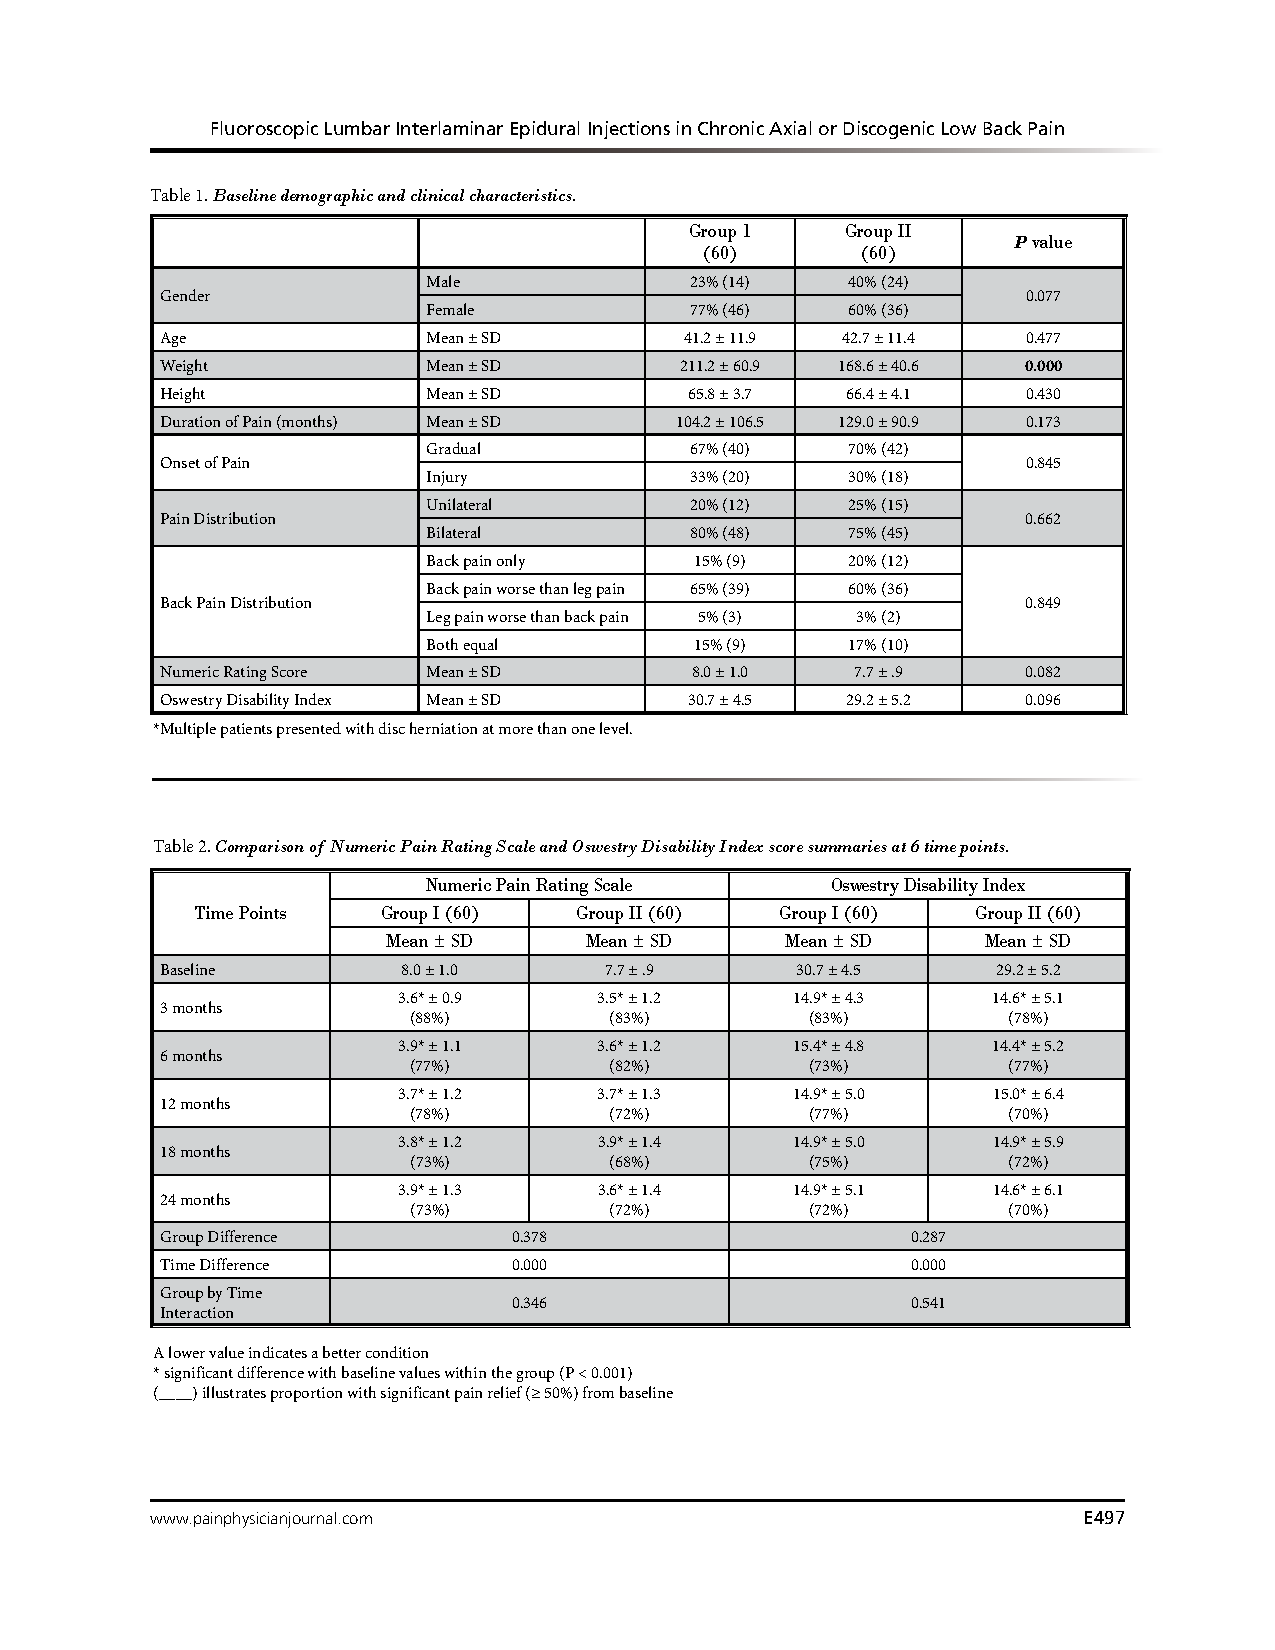
\includegraphics[trim={1.5cm 15.3cm 1.5cm 3.5cm},clip,width=0.8\textwidth]{Plots/Statisztika-ketmintas-tablak.pdf}
		\end{center}
		
	
	\subsubsection{Age variable}
	
	\begin{enumerate}[a)]
	\item The name of the appropriate test:	\hrulefill
	
		Why we can't apply paired $t$-test? \hrulefill
	\item H$_0$:	\hrulefill

		 H$_A$:	\hrulefill
	\item Assumptions of the test:	\hrulefill
			\\
			Normality fulfillment: \hrulefill
			\\
			Equal variances fulfillment: \hrulefill
			
	\item \emph{Descriptive statistics}: 
		%
		\hrulefill
		
	\item Is there a significant difference?\hrulefill\quad Why? \hrulefill
	
	\item Check the $p$-value with R. Was the chosen method appropriate? \hrulefill
	\end{enumerate}
	
	
		\subsubsection{Duration of Pain  variable}
		
		\begin{enumerate}[a)]
		\item The name of the appropriate test:	\hrulefill
		
			Why we can't apply paired $t$-test? \hrulefill
		\item H$_0$:	\hrulefill
	
			 H$_A$:	\hrulefill
		\item Assumptions of the test:	\hrulefill
				\\
				Normality fulfillment: \hrulefill
				\\
				Equal variances fulfillment: \hrulefill
				
		\item \emph{Descriptive statistics}: 
		%
			\hrulefill
			
		\item Is there a significant difference?\hrulefill\quad Why? \hrulefill
		
		\item Check the $p$-value with R. Was the chosen method appropriate? \hrulefill
		\end{enumerate}

\clearpage
\subsection{Compare beers}
Using \data{BEER.csv} datafile,  compare the calorie content and prices of \emph{LIGHT} and \emph{NONLIGHT} american beers  (variables \variable{LIGHT} and \variable{CALORIES})!
The population means of light and nonlight beers are the same?

\subsubsection{Calories}
	\begin{enumerate}[a)]

	\begin{multicols}{2}
	\item Applied test:
	
	\hrulefill
	\item H$_0$: \hrulefill\quad H$_A$: \hrulefill
	
		
	\item Assumption(s) of the test: \hrulefill

		Fulfillment(s)? \hrulefill 
		
		 \hrulefill

		\item Descriptive statistics
		\begin{center}\small
			\begin{tabular}{r|C{2cm}|C{2cm}}
			\toprule
						& light & nonlight\\
			\midrule
			sample size	&&\\
			mean		&&\\
			SD		&&\\
			SE			&&\\
			\bottomrule
			\end{tabular}
		\end{center}
	\end{multicols}

	\item \emph{Result}
	
		Test-statistics: \hrulefill\quad df: \hrulefill\quad $p$-value: \hrulefill
		
		Is there a significant difference?? \rule{5em}{0.4pt} Why? \hrulefill
	\end{enumerate}
	
\subsubsection{Prices}
	\begin{enumerate}[a)]
		\begin{multicols}{2}
	


	\item Applied test:
	
	\hrulefill
	\item H$_0$: \hrulefill\quad H$_A$: \hrulefill
	
		
	\item Assumption(s) of the test: \hrulefill

		Fulfillment(s)? \hrulefill 
		
		 \hrulefill

		\item Descriptive statistics
		\begin{center}\small
			\begin{tabular}{r|C{2cm}|C{2cm}}
			\toprule
						& light & nonlight\\
			\midrule
			sample size	&&\\
			mean		&&\\
			SD		&&\\
			SE			&&\\
			\bottomrule
			\end{tabular}
		\end{center}
	\end{multicols}
	\item \emph{Result}
	
		Test-statistics: \hrulefill\quad df: \hrulefill\quad $p$-value: \hrulefill
		
		Is there a significant difference?? \rule{5em}{0.4pt} Why? \hrulefill
	\end{enumerate}
	
\section{Calculations with R}

\subsection{Open the file \data{befafter.csv}. A study was conducted to determine weight loss, body composition, etc. in obese women before and after 12 weeks of treatment with a very-low-calorie diet. Column \variable{BEFORE} and \variable{AFTER} contain weights of 9 women. We wish to know if these data provide sufficient evidence to allow us to conclude that the treatment is effective in causing weight reduction in obese women. Let $\alpha= 0.05$}

		
\begin{enumerate}[a)]

\item The name of the appropriate test:	 \hrulefill

	H$_0$:	 \hrulefill\\
		 H$_A$:	 \hrulefill


\begin{multicols}{2}
		\begin{center}\small
		\begin{tabular}{lC{2cm}C{2cm}}
			\toprule	
				\textit{}		& mean & SD\\
			\midrule
			Before &&\\
			After  &&\\
			difference &&\\
			\bottomrule
		\end{tabular}\medskip
	\end{center}

	 95\% CI for the difference:  \hrulefill
	%

	 $t =$ 	 \hrulefill\quad degrees of freedom = 	 \hrulefill\quad $t_\alpha$=	\hrulefill	
	 
	 $p$-value = \hrulefill 
	

\end{multicols}
	
	\item	Decision: \hrulefill

\end{enumerate}


	
\subsection{Open the file \quest!\\ Compare the mean body mass of boys and girls (at 5\% level).}
	

	\begin{enumerate}[a)]

	\item The name of the appropriate test:\hrulefill
	\item H$_0$:	\hrulefill
	
		H$_A$:	\hrulefill
		
	\item Assumptions: 	\hrulefill
	\end{enumerate}
	
		\begin{multicols}{2}
		\begin{center}
			\begin{tabular}{r|C{2cm}|C{2cm}}
			\toprule
						& boys & girls\\
			\midrule
			sample size	&&\\
			mean		&&\\
			SD		&&\\
			SE			&&\\
			\bottomrule
			\end{tabular}
		\end{center}

\subsubsection*{Equality of variances $\alpha=5\%$}
		\begin{enumerate}[a)]
		\item $p$-value: \hrulefill	
		\item Decision about the equality of variances:	
		
		\hrulefill
		\end{enumerate}
		\end{multicols}
\subsubsection*{Equality of population means $\alpha=5\%$}
		\begin{enumerate}[a)]
		\item $t=$ \hrulefill \quad df?	\hrulefill\quad			$p=$ \hrulefill
		\item 95\% CI of the difference: \hrulefill
		\item Decision about the equality of population means: \hrulefill

			Conclusion: \hrulefill		
		\end{enumerate}



\section{Homework}
%	
%\subsection{The systolic blood pressure of 6 patients was measured before and after a new drug. The mean of the sample differences is 6 mmHg, the standard error of the differences is 4.65. Is there a significant change in blood pressure at 5\% and at 1\% level?}
%
%	\begin{minipage}{0.45\textwidth}
%	$\alpha=5\%$
%	
%		\begin{enumerate}[a)]
%		\item Appropriate test: \hrulefill
%		\item H$_0:$	 \hrulefill
%
%			 H$_A$:	 \hrulefill
%		\item t: 	 \hrulefill
%
%			degrees of freedom: \hrulefill 
%
%			critical value: \hrulefill
%		\item Decision: 	 \hrulefill
%
%				Conclusion: \hrulefill
%		\end{enumerate}
%	\end{minipage}
%	\hfill
%	\begin{minipage}{0.45\textwidth}
%		$\alpha=1\%$
%		
%		\begin{enumerate}[a)]
%		\item Appropriate test: \hrulefill
%		\item H$_0:$	 \hrulefill
%
%			 H$_A$:	 \hrulefill
%		\item t: 	 \hrulefill
%
%			degrees of freedom: \hrulefill 
%
%			critical value: \hrulefill
%		\item Decision: 	 \hrulefill
%
%				Conclusion: \hrulefill
%		\end{enumerate}
%	\end{minipage}

\subsection{The body mass of 16 patients was measured before and after a special diet. The mean of the sample differences is 5 kg, the standard deviation of the differences is 2.5. Is there a significant change in body mass at 5\% and at 1\% level?}
	
	\begin{multicols}{2}
	
	$\alpha=5\%$
		\begin{enumerate}[a)]
		\item Appropriate test: \hrulefill
		
				H$_0:$	 \hrulefill
				H$_A$:	 \hrulefill
	\item t: 	 \hrulefill

			degrees of freedom: \hrulefill  \quad 
			critical value: \hrulefill
		\item Decision: 	 \hrulefill

				Conclusion: \hrulefill
		\end{enumerate}
	\columnbreak
			$\alpha=1\%$
		\begin{enumerate}[a)]
		\item Appropriate test: \hrulefill

			H$_0:$	 \hrulefill
			 H$_A$:	 \hrulefill
		\item t: 	 \hrulefill

			degrees of freedom: \hrulefill  \quad 
			critical value: \hrulefill

		\item Decision: 	 \hrulefill

				Conclusion: \hrulefill
		\end{enumerate}
	\end{multicols}	

\subsection[LWTBWT.csv]{Open the file \data{LWTBWT.csv} and compare the mean body weight of newborn babies (variable \variable{BWT}) by smoking habits of the mother (variable  \variable{SMOKE} 0 no, 1 yes)} 


\subsection[ANTHROPOMETRICS.csv]{Open the file \data{ANTHROPOMETRICS.csv} and compare the body height of boys and girls. Find other variables to be compared and find the appropriate test.}

\subsection[CALC.csv]{Open the file \data{CALC.csv}! Here systolic blood pressures are given before and after a calcium treatment in two groups. Find problems where paired $t$-tests can be used. Find problems where two-sample $t$-tests can be used. }

\subsection[NEWDRUG.csv]{Open the file \data{NEWDRUG.csv} and find problems where paired $t$-tests can be used. Find problems where two-sample $t$-tests can be used.}

	\chapter[Correlation and regression]{Correlation and\\regression}

\section[Relation of mass and height]{In a dataset measuring people’s height and mass, let’s examine the relationship between height and mass.}



\begin{multicols}{2}
	\begin{enumerate}[a)]
	\item Based on the plot, what would you say about the linear relationship?

		\begin{itemize}
		\item direction: 	\hrulefill	
		\item strength: \hrulefill
		\end{itemize}
	
	\item The correlation coefficient calculated from the data is $r = 0.6556$.

	
	What does the \dots of the correlation coefficient indicate?
	
		\begin{itemize}
		\item absolute value: \hrulefill	% TODO
		\item sign: 	\hrulefill
		\end{itemize}

	\item How would you describe this linear relationship based on the correlation coefficient? \hrulefill	
	\item Why do we need to test whether the correlation coefficient is significant? \hrulefill	
	
		\columnbreak
			\begin{center}
		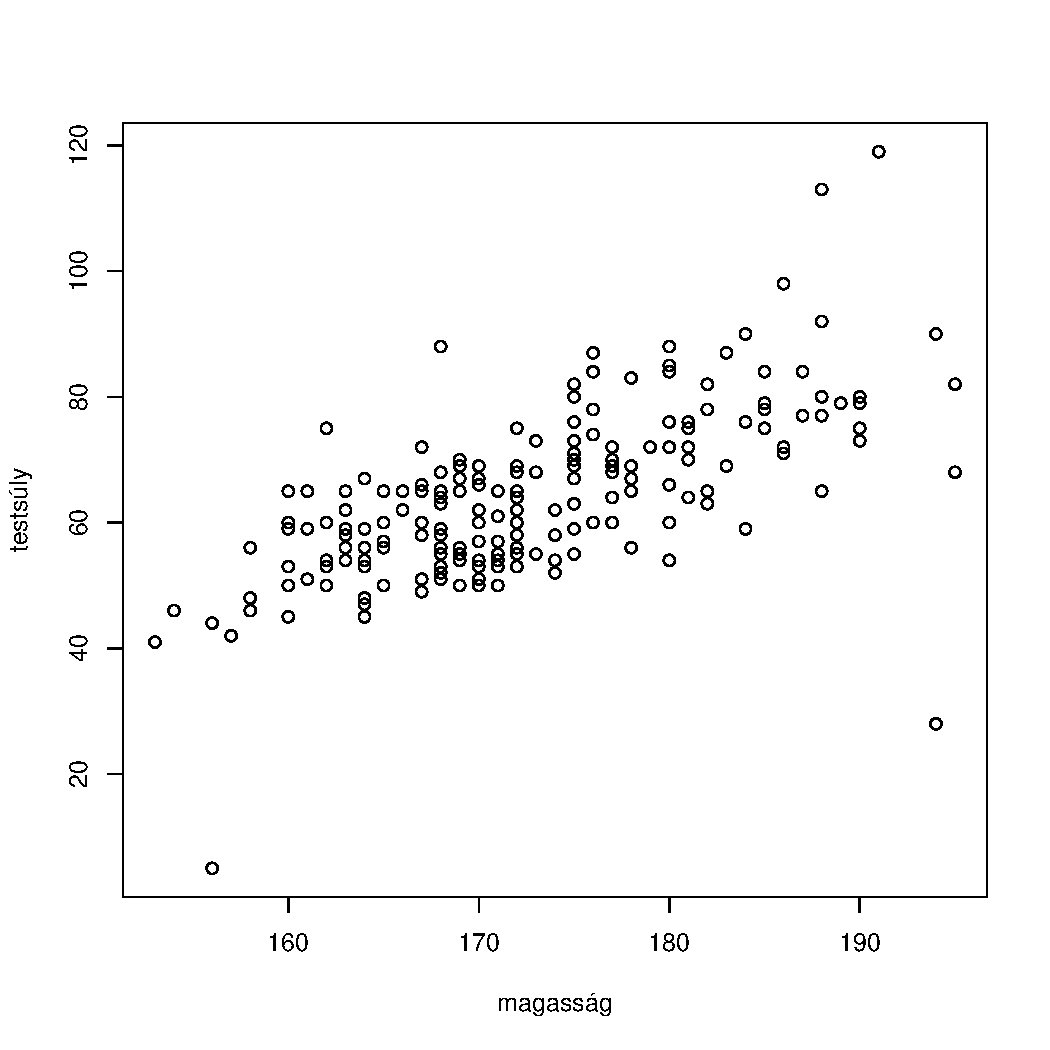
\includegraphics[width=0.48\textwidth]{Korrelacio-1}
		\end{center}
	\end{enumerate}
\end{multicols}

	
\subsection*{Significance test for the correlation coefficient ($n = 206$)}  
\begin{enumerate}[a)]\setcounter{enumi}{4}
\item Null hypothesis: \hrulefill		
	
	 Alternative hypothesis: \hrulefill		
\item t-value of the correlation: \hrulefill	
\item Degrees of freedom:	\hrulefill	 \quad Critical value: ($t_\alpha$): 	\hrulefill	
\item Decision and conclusion: \hrulefill		
\item The equation of the regression line: $y = 0,9698\cdot x - 103,147$ ($\textrm{mass} = 0,9698 \cdot \textrm{height}- 103,147$)

	Meaning: 	\hrulefill

	 What mass ''belongs'' to someone whose height is 160 cm, based on the regression line? \hrulefill	


\item Coefficient of determination

$$r^2 = \frac{ \textrm{squares}_{Regression} }{ \textrm{squares}_{Total} } = 0.4299$$

Meaning: 	\hrulefill
\subsection*{Find these values in the R output.}

\lstinputlisting[float=!h,frame=tblr]{Code/06-correlation1.txt}



\subsection*{Significance tests for the coefficients of the regression line}
\item Null hypothesis of the regression coefficient: \hrulefill\quad $t$-value: \hrulefill\quad	df: \hrulefill

$p$-value:	\hrulefill\quad significance:	\hrulefill\quad

\item Null hypothesis of the constant term: \hrulefill\quad $t$-value: \hrulefill\quad df: \hrulefill

$p$-value:	\hrulefill\quad significance:	\hrulefill\quad

\end{enumerate}
\clearpage




\section[Connection of money spent on alcohol and tobacco]{A British survey examined the connection of money spent on alcohol and tobacco in 10 different regions of GBR. The correlation coefficient of money spent on alcohol and tobacco is $r = 0.784$. Test whether this is significantly different from 0 at 5\% level. (\data{S:/R/alcohol.csv})}

\subsection*{Hand calculation}
\begin{enumerate}[a)]
\item H$_0$: \hrulefill		


 H$_A$: \hrulefill		
 
 Assumption(s): \hrulefill
\item $t$-value: \hrulefill\quad df:	\hrulefill	 \quad Critical value ($t_\alpha$): 	\hrulefill	
\item Decision: \hrulefill

	 Conclusion: \hrulefill

\subsection*{We ran the previous example in R. Interpret the results.}

\lstinputlisting[float=!h,frame=tblr]{Code/06-correlation2.txt}
\begin{flushright}
	\vspace{-18em}
	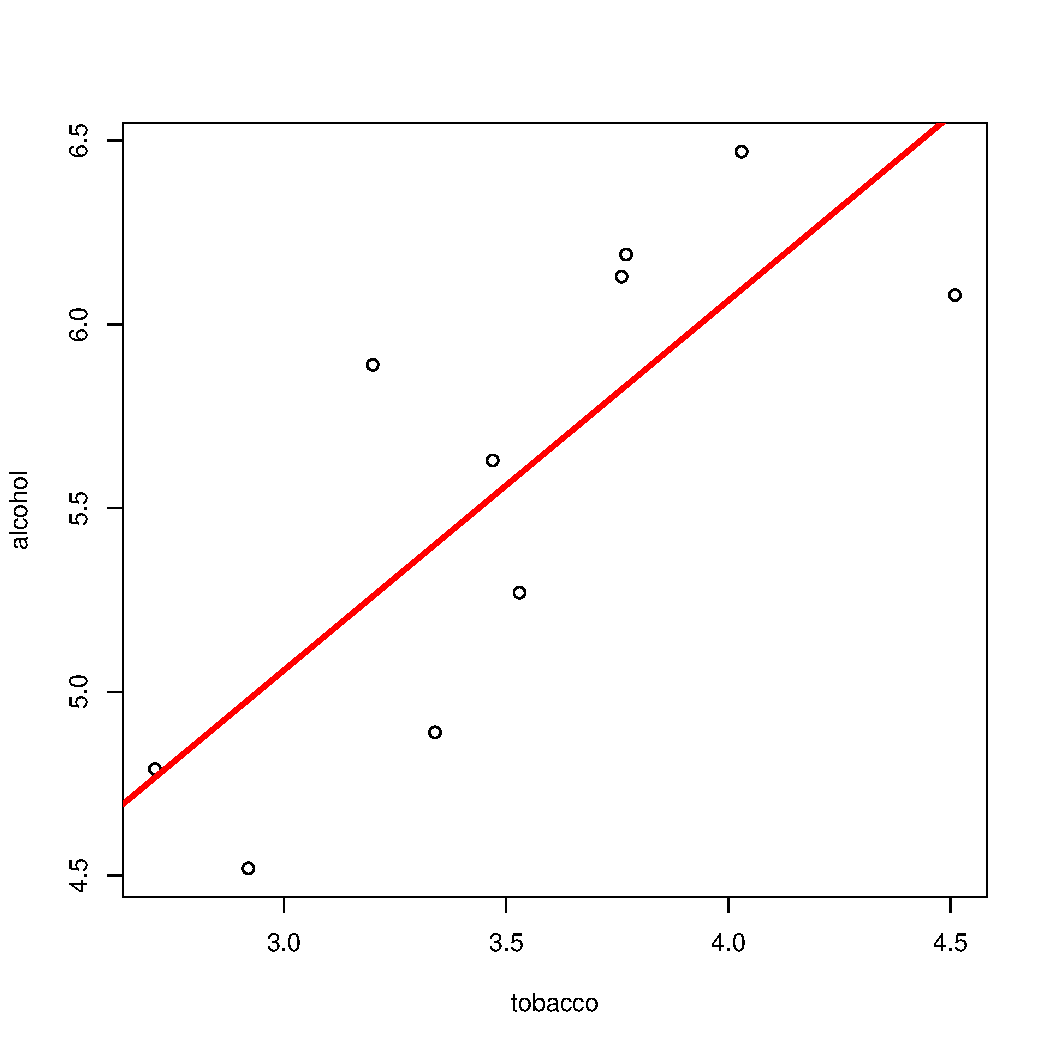
\includegraphics[width=0.3\textwidth]{Korrelacio-2}\hspace*{3em}
\end{flushright}

\item Correlation coefficient ($r$): \hrulefill\quad 	 Coefficient of determination $r^2$: \hrulefill
\item $t$:\hrulefill\quad df: \hrulefill\quad	 $p$-value:	\hrulefill
\item Conclusion to the direction and strength of the linear relationship: 	\hrulefill
\item Equation of the regression line: \hrulefill


\item Significance of the regression coefficients (use R to answer this question): \hrulefill
\end{enumerate}
\clearpage

\section{Is the correlation coefficient significantly different from 0 at 5\% level?}

 H$_0$: \hrulefill\quad H$_A$: \hrulefill		
\subsection{Based on $n = 5$ pairs of observations, the correlation coefficient is $r = 0.8$.}
\begin{enumerate}[a)]
\item $t$-value: \hrulefill\quad df:	\hrulefill	 \quad Critical value ($t_\alpha$): 	\hrulefill	
\item Decision: \hrulefill

	Interpretation (is there a contradiction?): \hrulefill
\end{enumerate}

\subsection{Based on $n = 500$ pairs of observations, the correlation coefficient is $r = 0.2$.}
\begin{enumerate}[a)]
%\item H$_0$: \hrulefill\quad H$_A$: \hrulefill		
\item $t$-value: \hrulefill\quad df:	\hrulefill	 \quad Critical value ($t_\alpha$): 	\hrulefill	
\item Decision: \hrulefill

	 Interpretation (is there a contradiction?): \hrulefill
\end{enumerate}

\subsection{Based on $n = 15$ pairs of observations, the correlation coefficient is $r = -0.8$.}

\begin{enumerate}[a)]
%\item H$_0$: \hrulefill\quad H$_A$: \hrulefill		
\item $t$-value: \hrulefill\quad df:	\hrulefill	 \quad Critical value ($t_\alpha$): 	\hrulefill	
\item Decision: \hrulefill

 Interpretation: \hrulefill
\end{enumerate}

\section{Practice with R}
\subsection{Open the \quest data file. Examine the relationship between \variable{height} and \variable{mass}. Create a scatter plot. }
\begin{enumerate}[a)]
\item Correlation coefficient $r$: \hrulefill\quad	 Coefficient of determination $r^2$:	 \hrulefill
\item % Correlation coefficient szignifikanciája
%
	 $t$: \hrulefill\quad	 df: \hrulefill\quad $p$:	 \hrulefill

 Decision: \hrulefill
%	Conclusion to the direction and strength of the linear relationship: \hrulefill
\item Equation of the regression line: \hrulefill
\item Significance of the regression coefficients: \hrulefill
\end{enumerate}

\subsection{Open the data file \data{anthropometrics.csv}! Examine the connection between the first and second measurement of weight. Create a scatter plot.}
%Készítsünk ábrát!
\begin{enumerate}[a)]
\item Correlation coefficient $r$: \hrulefill\quad	 Coefficient of determination $r^2$:	 \hrulefill
\item %Correlation coefficient szignifikanciája 
$t$: \hrulefill\quad	 df: \hrulefill\quad $p$:	 \hrulefill

 Decision: \hrulefill
%	Conclusion to the direction and strength of the linear relationship: \hrulefill
\item Equation of the regression line: \hrulefill
\item Significance of the regression coefficients: \hrulefill
\end{enumerate}

\subsection{ Open the data file \data{anthropometrics.csv}! Examine the linear association between height and hip circumference. Create a scatter plot.}
\begin{enumerate}[a)]
\item Correlation coefficient $r$: \hrulefill\quad	 Coefficient of determination $r^2$:	 \hrulefill
\item %Correlation coefficient szignifikanciája 
%
	 $t$: \hrulefill\quad	 df: \hrulefill\quad $p$:	 \hrulefill

 Decision: \hrulefill
\item Equation of the regression line: \hrulefill
\item Significance of the regression coefficients: \hrulefill
\end{enumerate}

	\chapter[$\chi^2$-test for independence]{$\chi^2$-test for\\ independence}
\section[Medical check-up vs. gender]{In a (hypothetical) study, the relationship between gender and participation in annual medical check-ups was examined. The results are summarized in the following $2\times 2$ contingency table (observed frequencies).}

\begin{center}\small
	\begin{tabular}{c|C{2cm}C{2cm}|c}
	\toprule
	\multicolumn{4}{c}{\textit{Observed frequencies}}\\
	\midrule
		&\multicolumn{2}{c|}{\textbf{Medical check-ups}}\\
		&\multicolumn{2}{c|}{\textbf{within the last 1 year}}	\\
	\textbf{GENDER}	&\textbf{yes}	&\textbf{no}	&Total\\
	\midrule
	\textbf{male}	&15	&40	&55\\
	\textbf{female}		&25	&20	&45\\
	\midrule
	Total&40	&60	&100\\
	\bottomrule
	\end{tabular}
	\hfill	\begin{tabular}{c|C{2cm}C{2cm}|c}
	\toprule
	\multicolumn{4}{c}{\textit{Expected frequencies}}\\
	\midrule
		&\multicolumn{2}{c|}{\textbf{Medical check-ups}}\\
		&\multicolumn{2}{c|}{\textbf{within the last 1 year}}	\\
		\textbf{GENDER}	&\textbf{yes}	&\textbf{no}	&Total\\
		\midrule
		\textbf{male}	&	&	&55\\
		\textbf{female}		&	&	&45\\
		\midrule
		Total&40	&60	&100\\
		\bottomrule
		\end{tabular}
\end{center}

\noindent\textbf{Is participation in routine medical check-ups independent of gender at the 5\% significance level?}
 
\begin{enumerate}[a)]
\item \textit{Participation rate among}  

	males: \hrulefill \quad females: 	\hrulefill
\item The name of the appropriate test  \hrulefill
\item H$_0$: \hrulefill 	

	H$_A$: \hrulefill


	 Assumption(s) of the test:  \hrulefill

$
\displaystyle	\chi^2 =\sum_i \frac{(\textrm{observed}_i-\textrm{expected}_i)^2}{\textrm{expected}_i}=
$

\item Degrees of freedom: (number of rows - 1)$\cdot$(number of columns - 1)= \hrulefill\quad	 Critical value: \hrulefill	
\item Decision: 	\hrulefill

	Conclusion: \hrulefill
\end{enumerate}

\section[Drug vs. side effect]{ Two medicines are being compared regarding a particular side effect, 60 similar patients are split randomly into two groups, one on each drug. The results are presented in the observed frequencies table}


\begin{center}\small
	\begin{tabular}{c|C{15mm}C{15mm}|c}
		\toprule
		\multicolumn{4}{c}{\textit{Observed frequencies}}\\
		\midrule
			&\multicolumn{2}{c|}{\textbf{SIDE EFFECT}}\\
		\textbf{DRUG}	&\textbf{yes}	&\textbf{no}	&Total\\
		\midrule
		\textbf{A}	&10	&20	&30\\
		\textbf{B}	&5	&25 &30\\
		\midrule
		Total	&15	&45	&60\\
		\bottomrule
	\end{tabular}
	\hfill
	\begin{tabular}{c|C{15mm}C{16mm}|c}
		\toprule
		\multicolumn{4}{c}{\textit{Expected frequencies}}\\
		\midrule
			&\multicolumn{2}{c|}{\textbf{SIDE EFFECT}}\\
		\textbf{DRUG}	&\textbf{yes}	&\textbf{no}	&Total\\
		\midrule
		\textbf{A}	&	&	&30\\
		\textbf{B}	&	& &30\\
		\midrule
		Total	&15	&45	&60\\
		\bottomrule
	\end{tabular}
\end{center}


\noindent\textbf{Are drug type and the occurrence of side effect independent at the 5\% level?}

\begin{enumerate}[a)]
\item \textit{Percentage of people who had side effect taking}  

	drug A: \hrulefill \quad
	drug B 	\hrulefill
\item The name of the appropriate test:  \hrulefill
\item H$_0$: \hrulefill 	

 H$_A$: \hrulefill



Assumption(s) of the test: \hrulefill


$
\displaystyle	\chi^2 =\sum_i \frac{(\textrm{observed}_i-\textrm{expected}_i)^2}{\textrm{expected}_i}=
$

\item Degrees of freedom: (number of rows - 1)$\cdot$(number of columns - 1)= \hrulefill\quad	 Critical value: \hrulefill	
\item Decision: 	\hrulefill

	Conclusion: \hrulefill
\end{enumerate}

\section[Voting vs. age]{In a certain town, there are about 10\ 000 eligible voters. A random sample of 500 eligible voters was chosen to study the relationship between age and participation in the last election. The results are summarized in the following 3$\times$2- contingency table}

%Egy bizonyos expectedosban kb. 10\,000 szavazásra jogosult él.  Egy 500~főből álló véletlen minta alapján vizsgálták az életkor és a legutóbbi szavazáson való részvétel közötti kapcsolatot.  Az eredményeket a következő 3$\times$2-es gyakorisági táblázat tartalmazza.}


\begin{center}\small
	\begin{tabular}{c|C{15mm}C{15mm}|c}
	\toprule
		\multicolumn{4}{c}{\textit{Observed frequencies}}\\
	\midrule
		&\multicolumn{2}{c|}{\textbf{PARTICIPATION}}\\
	\textbf{AGE GROUP}	&\textbf{yes}	&\textbf{no}	&Total\\
	\midrule
	\textbf{Under age 40}	& 90	& 60	& 150\\
	\textbf{40 -- 60}		& 130	& 70	& 200\\
	\textbf{Above age 60}	& 120	& 30	& 150\\
	\midrule
	Total				& 340	& 160	& 500\\
	\bottomrule
	\end{tabular}
	\hfill
	\begin{tabular}{c|C{15mm}C{15mm}|c}
	\toprule
		\multicolumn{4}{c}{\textit{Expected frequencies}}\\
	\midrule
		&\multicolumn{2}{c|}{\textbf{PARTICIPATION}}\\
	\textbf{AGE GROUP}	&\textbf{yes}	&\textbf{no}	&Total\\
	\midrule
	\textbf{Under age 40}	& 	& 	& 150\\
	\textbf{40 -- 60}	& 	& 	& 200\\
	\textbf{Above age 60}	& 	& 	& 150\\
	\midrule
	Total			& 340	& 160	& 500\\
	\bottomrule
	\end{tabular}
\end{center}

\noindent \textbf{Is there a relationship between age group and having voted in the last election ($\alpha = 0.05$)? }

\begin{enumerate}[a)]
\item \textit{Participation rate}  

	Under age 40: \hrulefill \quad
	Between age 40 and 60: 	\hrulefill\quad
	Above age 60: \hrulefill
\item The name of the appropriate test:  \hrulefill
\item H$_0$: \hrulefill 	

	 H$_A$: \hrulefill


Assumption(s) of the test: \hrulefill


$
\displaystyle	\chi^2 =\sum_i \frac{(\textrm{observed}_i-\textrm{expected}_i)^2}{\textrm{expected}_i}=
$

\item Degrees of freedom: (number of rows - 1)$\cdot$(number of columns - 1)= \hrulefill\quad	 Critical value: \hrulefill	
\item Decision: 	\hrulefill

	Conclusion: \hrulefill
\end{enumerate}

\section[Aspirin vs. thrombi]{The following observed frequency table shows the results of placebo and aspirin treatments in an experiment, with the number of people in each treatment group who did and did not develop thrombi. Decide whether the aspirin had an effect on thrombus formation.}


\begin{center}\small
	\begin{tabular}{c|C{2cm}C{2cm}|c}
	\toprule
		\multicolumn{4}{c}{\textit{Observed frequencies}}\\
	\midrule
		&\multicolumn{2}{c|}{\textbf{Developed thrombi?}}\\
						&\textbf{yes}	&\textbf{Nem}	&Total\\
	\midrule
	\textbf{Placebo}	&16	&4	&20\\
	\textbf{Aspirin}	&6	&14 &20\\
	\midrule
	Total			&22	&18	&40\\
	\bottomrule
	\end{tabular}
	\hfill
		\begin{tabular}{c|C{2cm}C{2cm}|c}
		\toprule
			\multicolumn{4}{c}{\textit{Expected frequencies}}\\
			\midrule
			&\multicolumn{2}{c|}{\textbf{Developed thrombi?}}\\
							&\textbf{yes}	&\textbf{Nem}	&Total\\
		\midrule
		\textbf{Placebo}	&	&	&20\\
		\textbf{Aszpirin}	&	& &20\\
		\midrule
		Total			&22	&18	&40\\
		\bottomrule
		\end{tabular}
\end{center}



\begin{enumerate}[a)]
\item \textit{The thrombus formation rate in the\dots}  

	placebo group: \hrulefill \quad 	aspirin group: \hrulefill
\item The name of the appropriate test:  \hrulefill
\item H$_0$: \hrulefill 	

	H$_A$: \hrulefill


 Assumption(s) of the test: \hrulefill

\item Test-statistic:  

$
\displaystyle	\chi^2 =\sum_i \frac{(\textrm{observed}_i-\textrm{expected}_i)^2}{\textrm{expected}_i}=
$

\item Degrees of freedom: (number of rows - 1)$\cdot$(number of columns - 1)= \hrulefill\quad	 Critical value: \hrulefill	
\item Decision: 	\hrulefill

	Conclusion: \hrulefill
\end{enumerate}


\section[Gender vs. pleased]{Examine the relationship between the answers of \variable{pleased} and \variable{gender}. Are the answers to the question ''Are you pleased with using a statistical software?'' independent of gender? Use the \quest dataset!}



\begin{center}\small
	\begin{tabular}{c|C{2cm}C{2cm}|c}
	\toprule
		\multicolumn{4}{c}{\textit{Observed frequencies}}\\
	\midrule
		&\multicolumn{2}{c|}{\textbf{PLEASED}}\\
	\textbf{GENDER}	&\textbf{yes}	&\textbf{no}	&Total\\
	\midrule
	\textbf{male}	&	& &\\
	\textbf{female}	&	& &\\
	\midrule
	Total			&	&	&\\
	\bottomrule
	\end{tabular}
	\hfill
		\begin{tabular}{c|C{2cm}C{2cm}|c}
		\toprule
			\multicolumn{4}{c}{\textit{Expected frequencies}}\\
			\midrule
			&\multicolumn{2}{c|}{\textbf{PLEASED}}\\
		\textbf{GENDER}	&\textbf{yes}	&\textbf{no}	&Total\\
		\midrule
		\textbf{male}	&	& &\\
		\textbf{female}	&	& &\\
		\midrule
		Total			&	&	&\\
		\bottomrule
		\end{tabular}
\end{center}



\begin{enumerate}[a)]
\item The name of the appropriate test:  \hrulefill
\item H$_0$: \hrulefill 	

	H$_A$: \hrulefill

 Assumption(s) of the test: \hrulefill

\item $\chi^2=$ \hrulefill\quad Degrees of freedom= \hrulefill\quad $p=$ \hrulefill
\item Fisher's exact $p$-value: \hrulefill 
\item Decision: 	\hrulefill
	
	Conclusion: \hrulefill
\end{enumerate}


\section[Gender vs. difficult]{Examine whether the answers to the question ''Is biostatistics difficult'' depend on gender.}



\begin{center}\small
	\begin{tabular}{c|C{2cm}C{2cm}|c}
	\toprule
		\multicolumn{4}{c}{\textit{Observed frequencies}}\\
	\midrule
		&\multicolumn{2}{c|}{\textbf{DIFFICULT}}\\
		\textbf{GENDER}	&\textbf{yes}	&\textbf{no}	&Total\\
	\midrule
	\textbf{male}	&	& &\\
	\textbf{female}	&	& &\\
	\midrule
	Total			&	&	&\\
	\bottomrule
	\end{tabular}
	\hfill
		\begin{tabular}{c|C{2cm}C{2cm}|c}
		\toprule
			\multicolumn{4}{c}{\textit{Expected frequencies}}\\
			\midrule
			&\multicolumn{2}{c|}{\textbf{DIFFICULT}}\\
		\textbf{GENDER}	&\textbf{yes}	&\textbf{no}	&Total\\
		\midrule
		\textbf{male}	&	& &\\
		\textbf{female}	&	& &\\
		\midrule
		Total			&	&	&\\
		\bottomrule
		\end{tabular}
\end{center}



\begin{enumerate}[a)]
\item The name of the appropriate test:  \hrulefill
\item H$_0$: \hrulefill 	

	H$_A$: \hrulefill


	 Assumption(s) of the test: \hrulefill

\item $\chi^2=$ \hrulefill\quad Degrees of freedom= \hrulefill\quad $p=$ \hrulefill
\item Fisher's exact $p$-value: \hrulefill 
\item Decision: 	\hrulefill

	 Conclusion: \hrulefill
\end{enumerate}



\section[Gender vs. eating habits]{Examine whether answers to the question ''How do you like to eat?'' depend on gender.}



\begin{center}\footnotesize
		\begin{tabular}{r|C{15mm}C{15mm}|c}
		\toprule
			\multicolumn{4}{c}{\textit{Observed frequencies}}\\
			\midrule
			&\multicolumn{2}{c|}{\textbf{GENDER}}\\
		\textbf{EATING}	&\textbf{male}	&\textbf{female}	&Total\\
		\midrule
		\textbf{I don't like to eat at all}	&	& &\\		
		\textbf{I don't like to eat}	&	& &\\
		\textbf{Indifferent}	&	& &\\
		\textbf{I like to eat}	&	& &\\
		\textbf{I like to eat very much}	&	& &\\
		\midrule
		Total			&	&	&\\
		\bottomrule
		\end{tabular}
	\hfill
	\begin{tabular}{r|C{15mm}C{15mm}|c}
		\toprule
			\multicolumn{4}{c}{\textit{Expected frequencies}}\\
			\midrule
			&\multicolumn{2}{c|}{\textbf{GENDER}}\\
		\textbf{EATING}	&\textbf{male}	&\textbf{female}	&Total\\
		\midrule
		\textbf{I don't like to eat at all}	&	& &\\		
		\textbf{I don't like to eat}	&	& &\\
		\textbf{Indifferent}	&	& &\\
		\textbf{I like to eat}	&	& &\\
		\textbf{I like to eat very much}	&	& &\\
		\midrule
		Total			&	&	&\\
		\bottomrule
		\end{tabular}
\end{center}



\begin{enumerate}[a)]
\item The name of the appropriate test:  \hrulefill
\item H$_0$: \hrulefill 	

	H$_A$: \hrulefill


Assumption(s) of the test: \hrulefill

\item $\chi^2=$ \hrulefill\quad Degrees of freedom= \hrulefill\quad $p=$ \hrulefill
\item Fisher's exact $p$-value: \hrulefill 
\item Decision: 	\hrulefill

	 Conclusion: \hrulefill
\end{enumerate}

	\chapter[Agreement, odds ratio and relative risk]{Agreement, odds ratio\\ and relative risk}


\section{Measure agreement (kappa)}
Two people (MN és VU) qualified psychiatric patients. Do  they agree? 

\noindent\textbf{Calculate the $\kappa$ (kappa)  statistics and interpret the reults!}

\begin{flushright}
\small Source:
Wongpakaran et al.: A comparison of Cohen’s Kappa and Gwet’s AC1 when calculating inter-rater reliability coefficients: a study conducted with personality disorder samples,  BMC Research Methodolgy 2013,13:61. \\
\url{http://www.biomedcentral.com/1471-2288/13/61}
\end{flushright}




\begin{minipage}{0.5\textwidth}
	\subsection{Avoidant} 
	$\kappa=$\rule{2cm}{0.4pt}\quad agreement: \rule{2cm}{0.4pt}

	\subsection{Dependent}
	$p_o=0.9474$, $p_e=0.8532$\medskip
	
	$\kappa=$\rule{2cm}{0.4pt}\quad agreement: \rule{2cm}{0.4pt}
	\subsection{Depressive}
	$p_o=0.8947$, $p_e=0.7431$\medskip
		
		$\kappa=$\rule{2cm}{0.4pt}\quad agreement: \rule{2cm}{0.4pt}
	\subsection{Schizoid}
	$p_o=0.8421$, $p_e=0.6371$\medskip
		
		$\kappa=$\rule{2cm}{0.4pt}\quad agreement: \rule{2cm}{0.4pt}
	\subsection{Total antisocial} 
	$p_o=0.8947$, $p_e=0.8116$\medskip
		
		$\kappa=$\rule{2cm}{0.4pt}\quad agreement: \rule{2cm}{0.4pt}
\end{minipage}	
\hfill
\begin{minipage}{0.4\textwidth}
	
	\begin{tabular}{lc|cc}
	\toprule
	%\textbf{PDs}
					& 			& \multicolumn{2}{c}{\textbf{Rater VU}} 	\\
					& \textbf{Rater MN}	& NO & YES\\
					\midrule
	Avoidant 		& NO		& 14 & 0\\
					& YES		& 0  & 5\\
					\midrule
	Dependent 		& NO		& 17 & 1\\
					& YES		& 0  & 1\\
				\midrule
	Depressive 		& NO		& 15 & 1\\
					& YES		& 1  & 2\\
				\midrule
	Schizoid 		& NO		& 13 & 2\\
					& YES		& 1  & 3\\
				\midrule
	Total  			& NO		& 16 & 1\\
	antisocial		& YES		& 1  & 1\\
					\bottomrule
	\end{tabular}

\end{minipage}

\clearpage
\section{Odds ratio (OR)}
Children's drug use and risk factors were examined in a retrospective (case-control) study. Examine and interpret the odds ratios in the following table and determine the significance based on the confidence intervals
%Egy vizsgálatban a gyermekek droghasználatát és annak rizikótényezőit vizsgálták retrospektív (eset-kontroll) vizsgálatban Az alábbi táblázat adatai alapján ellenőrizze az esélyhányadosokat, értelmezze őket és állapítsa meg a szignifikanciát a confidence interval alapján!


\begin{center}
	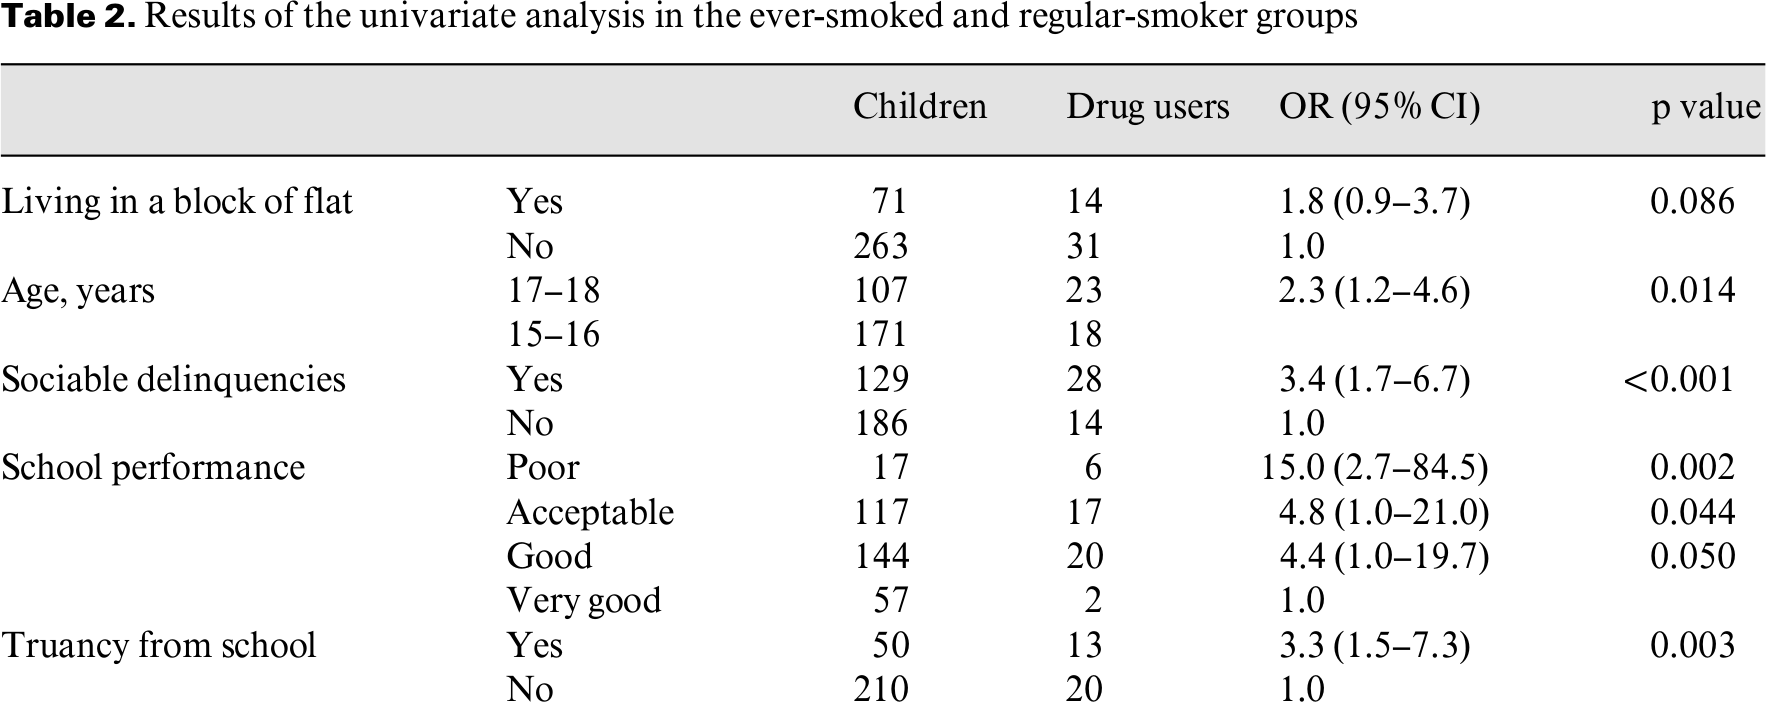
\includegraphics[width=0.9\textwidth]{G08-euraddict_table}
\end{center}


\begin{flushright}
\small Source: Nyári T.A., Herédi K. and Parker L.: Addictive Behaviour of Adolescents in Secondary Schools in Hungary.\\
	 Eur Addict Res 2005;11:38– 3 DOI:10.1159/00008141
\end{flushright}
Why did they calculate OR? \hrulefill


\subsection{Living in a block flat vs drug usage}
Table interpretation: in first row one can see that 14 children out 71 use drugs. In the second row 31 use druges out of 263. Create a 2$\times 2$ table and calculate the OR.
%az első sorban látható, hogy 71 gyerek közül 14 drogozik, a második sorban 263 gyerekből 31. Készítse el a 2x2-es táblázatot és számítsa ki az esélyhányadost (OR).

\begin{center}
		\begin{tabular}{r|C{15mm}C{15mm}|c}
		\toprule
			&\multicolumn{2}{c|}{\textbf{DRUG}}\\
		\textbf{Block flat}	&\textbf{yes}	&\textbf{no}	&Total\\
		\midrule
		\textbf{yes}	&	& &71\\		
		\textbf{no}	&	& &263\\
	%	\midrule
	%	Total			&	&	&\\
		\bottomrule
		\end{tabular}
\end{center}

\begin{enumerate}[a)]
\item The probability child use drug is
	\begin{itemize}
	\item when lives in block flat:  \rule{5cm}{0.4pt}
	\item when does not live in block flat: \rule{5cm}{0.4pt}
	\end{itemize}

\item  Quotient (OR)= \hrulefill

	Using the formula: \hrulefill

	Interpretation: \hrulefill
\item 95\% confidence interval: 	\hrulefill

\subsubsection*{Significance of odds ratio}
	\item H$_0$: \textsc{	\hrulefill}

			 H$_A$: \hrulefill
	\item Decision about significance based on CI: \hrulefill

	Decision based on $p$-value:	\hrulefill
\end{enumerate}

\subsection[School performance]{School performance. Compare the good and very good category with the drug usage. Calculate OR!}

\begin{center}
		\begin{tabular}{r|C{15mm}C{15mm}|c}
		\toprule
		\textbf{SCHOOL}		&\multicolumn{2}{c|}{\textbf{DRUG}}\\
		\textbf{PERFORMANCE}	&\textbf{yes}	&\textbf{no}	&Total\\	
		\midrule
		\textbf{good}	&	& &\\		
		\textbf{very good}	&	& &\\
	%	\midrule
	%	Total			&	&	&\\
		\bottomrule
		\end{tabular}
\end{center}

\begin{enumerate}[a)]

\item The probability that a child use drug if s/he is 
	\begin{itemize}
	\item good:  \rule{5cm}{0.4pt}
	\item very good: \rule{3.8cm}{0.4pt}
	\end{itemize}


\item  Quotient (OR)= \hrulefill

	Using the formula: \hrulefill

	Interpretation: \hrulefill
\item 95\% confidence interval: 	\hrulefill

\subsubsection*{Significance of odds ratio}
	\item H$_0$: \textsc{	\hrulefill}

			 H$_A$: \hrulefill
	\item Decision about significance based on CI: \hrulefill

	Decision based on $p$-value:	\hrulefill
\end{enumerate}

\subsection[Truancy]{Truancy from school and drug usage
Create 2$\times$2-es table and calculate OR.}

\begin{center}
		\begin{tabular}{r|C{15mm}C{15mm}|c}
		\toprule
			&\multicolumn{2}{c|}{\textbf{DRUG}}\\
		\textbf{TRUANCY}	&\textbf{yes}	&\textbf{no}	&Total\\
		\midrule
		\textbf{yes}	&	& &\\		
		\textbf{no}	&	& &\\
%		\midrule
%		Total			&	&	&\\
		\bottomrule
		\end{tabular}
\end{center}

\begin{enumerate}[a)]
\item The probability that a child use drug if he 
	\begin{itemize}
	\item plays truant:  \rule{5cm}{0.4pt}
	\item does not play truant: \rule{4.2cm}{0.4pt}
	\end{itemize}


\item  Quotient (OR)= \hrulefill

	Using the formula: \hrulefill

	Interpretation: \hrulefill
\item 95\% confidence interval: 	\hrulefill

\subsubsection*{Significance of odds ratio}
	\item H$_0$: \textsc{	\hrulefill}

			 H$_A$: \hrulefill
	\item Decision about significance based on CI: \hrulefill

	Decision based on $p$-value:	\hrulefill
\end{enumerate}




\section{Relative risk (RR)}
In a prospective study risks of respiratory complications were examined.% Examine the relative risks and $p$-values
%Egy prospektív vizsgálatban gyermekek altatása során fellépő kockázati tényezők rizikófaktorait vizsgálták. Ellenőrizzük a táblázat alapján a kapott relatív kockázatokat és $p$-értékeket!


\begin{center}
	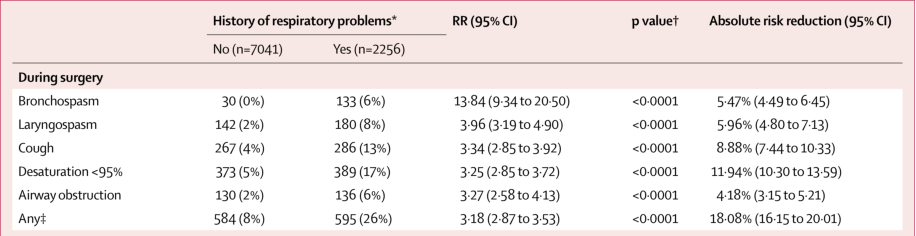
\includegraphics[width=\textwidth]{G08-RR_cikk_tabla}
\end{center}
\begin{flushright}
\small
Source: Britta S von Ungern-Sternberg és mtsai: Risk assessment for respiratory complications in paediatricanaesthesia:
a prospective cohort study. The Lancet, Vol 376 September 4, 2010, 773-783
\end{flushright}

\noindent Why did they calculate relative risk? \hrulefill\bigskip



\noindent\textbf{Examine using the table whether a respiratory problems (=yes) causes  more frequent brochospasmus complication!
Calculate a 2$\times$2-es táble and RR!}

\begin{center}
		\begin{tabular}{r|C{15mm}C{15mm}|c}
		\toprule
		\textbf{RESPIRATORY}	&\multicolumn{2}{c|}{\textbf{COMPLICATION}}\\
		\textbf{PROBLEMS}			&\textbf{yes}	&\textbf{no}	&Total\\
		\midrule
		\textbf{yes}	& 133	& & 2256\\		
		\textbf{no}	& 30	& & 7041\\
	%	\midrule
	%	Total		&		& &\\
		\bottomrule
		\end{tabular}
\end{center}


\begin{enumerate}[a)]
\item The risk of having complication if patient 
	\begin{itemize}
	\item had respiratory problems before: \rule{5cm}{0.4pt}
	\item did not have respiratory problems before: \rule{4.2cm}{0.4pt}
	\end{itemize}

\item Quotient (RR)= \hrulefill

	 Using the formula: \hrulefill

	Interpretation: 	\hrulefill
\item 95\% confidence interval of the relative risk: 	\hrulefill

\subsubsection*{Significance of the relative risk}
	\item H$_0$: \textsc{	\hrulefill}

		H$_A$: \hrulefill
	\item Decision about significance based on CI: \hrulefill

	Decision based on $p$-value:	\hrulefill
\end{enumerate}



	\chapter[Further problems]{Type of problems\\ not practiced during the semester}

\section{Fourfold (2$\times$2) tables}
\begin{enumerate}
\item In a study of measurement of agreement, the observed and expected probabilities were 0.85 and 0.5, respectively. Calculate the kappa statistic! 
\item In a study 40 HPV positive tests of 50 abnormal cervical samples and 10 HPV positive tests of 60 normal cervical samples were detected. Calculate the odds ratio! 
\item The risk of HPV infection for smokers was measured in a study. The calculated odds ratio was 1.58 with 95\% CI [1.061 - 2.398]. We decide... 
\item The risk of HPV infection for smokers was measured in a study. The calculated odds ratios was 1.58 with 95\% CI [0.961 - 2.598]. We decide ... 
\item In a study 8 HPV positive tests of 20 abnormal cervical samples and 10 HPV positive tests of 20 normal cervical samples were detected. Calculate the odds ratio! 
\end{enumerate}

\section{Nonparametric tests}
\begin{enumerate}
\item Find the ranks to the following data: 199, 126, 81, 68, 112, 112.

\end{enumerate}

\section{Survival analysis}
\begin{enumerate}
\item In a study the average period of time of free of disease was 3.1 year and SE=0.44. Compare this result to the reference 2.2 years of survival rate using a 95\% confidence interval!
\item In a study the average period of time of free of disease was 3.1 year and SE=0.44. Compare this result to the reference 2.2 years of survival rate! What is the null hypothesis ? 
\item In a cohort study the first year the interval survival rate was 0.99. In the following four years the annual interval survival rates were 0.98, 0.97, 0.96 and 0.95, respectively. Calculate the 5-year cumulative survival rate!
\item In a cohort study the first year the interval survival rate was 0.90. In the following four years the annual interval survival rates were 0.90, 0.90, 0.90 and 0.90, respectively. Calculate the 5-year cumulative survival rate!
\end{enumerate}

	
	\chapter{Summary of the methods}
%\fancyhead[LO,RE]{\textsc{Summary of the methods}}

\begin{enumerate}
\item\label{both-cont}
 both are continuous (measured on the same subject):
 
 	\begin{enumerate}
	\item comparing the means of variables – the same thing about the same subjets, examining mean change: \textbf{paired t-test}
	\item  examining relationships between variables: \textbf{correlation, regression}
	\end{enumerate}
\item\label{one-cont} one continuous dependent variable divided into independent groups according to another, categorical variable: (that is, comparing means of groups)

	\begin{enumerate}
	\item number of groups=2: \textbf{two-sample t-test} (Independent t-test)
	\item number of groups>2: \textbf{One-way ANOVA} (Analysis of Variance)
	\end{enumerate}
\item both are categorical: examination of contingency tables, \textbf{$\chi^2$ test}
\end{enumerate}

\noindent In \ref{both-cont}. and \ref{one-cont}. we assumed that the samples come from normal distribution. If this assumption does not hold or we have ordered data, use \textbf{nonparametric methods based on ranks}.

\vfill
\section{Manual calculation}

\subsection{Effect of a new drug}
To test the effect of a new drug, the temperature was measured on the same 10 patients before and after the treatment. The mean of the differences is = 0.6, the standard deviation of the differences is SD=0.4062. Test whether the drug is effective or not; i.e., test whether the change in mean is different from 0 at $\alpha$=0.05 level.

\begin{enumerate}[a)]
	\item To test the effect of the drug, what is the appropriate test?\hrulefill

	Assumption(s)?\hrulefill

	\item 
	State the null and the alternative hypothesis
		
		H$_0$:	\hrulefill\\
		H$_A$:	\hrulefill

	\item Find the degrees of freedom: \hrulefill
		\quad
	standard error: \hrulefill


	test statistic: \hrulefill
		\quad
	critical value: \hrulefill

	\item Decide whether the difference is significant or not: \hrulefill


		State a conclusion: \hrulefill

	\item \emph{Alternative solution using confidence interval}

	Find the 95\% confidence interval: \hrulefill

	Decide whether the difference is significant or not: \hrulefill

	Conclusion: \hrulefill
\end{enumerate}


\subsection{Drug side effect}
Two medicines are being compared regarding a particular side effect; 100 similar patients are split randomly into two groups, one of each group. In the group of drug A, 10 side effects were observed while in the group of drug B only 2 side effects were observed. Test whether drug and side effects are independent!\bigskip

	\begin{tabular}{c|cc|c}
	\toprule
		&\multicolumn{2}{c|}{\textbf{SIDE EFFECTS}}\\
	\textbf{DRUG}	&\textbf{yes}	&\textbf{no}	&{\color{white} Total}\\
	\midrule
	\textbf{A}	&	&	&\\
	\textbf{B}	&	&	&\\
	\midrule
				&		&\\
	\bottomrule
	\end{tabular}
\begin{enumerate}[a)]
	\item Give the percentage of side effects in 
	
		group A: \hrulefill\quad group B:  \hrulefill
	\item What is the appropriate test? 
	
		\hrulefill 
		

			Assumption(s) of the test:
		
		\hrulefill
	\item State the null and the alternative hypothesis
	
	H$_0$: 	\hrulefill 	\\
	H$_A$: \hrulefill 	
	
\item
	Find the test statistic: \hrulefill
	
\item
	Find the degrees of freedom: 	\hrulefill \quad Critical value ($\alpha=0.05$): \hrulefill 	


	\item Decide whether the difference is significant or not:\\
	
	 \hrulefill 	
	
	\item
	State a conclusion:
	
	 \hrulefill 	
	
	
	\end{enumerate}
	
	
\subsection{Association}
Based on 11 pairs of data, the coefficient of correlation is r=0.8. Is the correlation significant at 5\% level? What is your opinion about the direction and about the strength of the association? 	


\begin{enumerate}[a)]
	\item State the null and the alternative hypothesis
	
	H$_0$: 	\hrulefill 	\\
	H$_A$: \hrulefill 	
	
	\item Find the test statistic: \hrulefill
	
	\item Find the degrees of freedom: 	\hrulefill \quad Critical value: \hrulefill 	


	\item		Decision
	
	 \hrulefill 	
	
	\item
Interpretation
	
	 \hrulefill 	
	
	
	\end{enumerate}
	
	
	\vfill\clearpage
	 	
\section{Calculation using R}

Open the file \data{quest2016.csv}. This file contains data of first year medical students.
\subsection{Examine the relationship between ideal body mass and body mass}
Examine the relationship between the body mass (\variable{mass}) and the ideal body mass (\variable{ideal\_mass})! Let the present mass be the independent variable. Is there a linear relationship between body mass at present and ideal body mass?


\begin{enumerate}[a)]
	\item The name of the appropriate test:	
				\hrulefill 
				
		Assumption(s) of the test: \hrulefill
				
	\item	State the null and the alternative hypothesis
			
			H$_0$: 	\hrulefill 	\\
			H$_A$: \hrulefill 	
	\item
	
		$r=$  \rule{15mm}{.4pt}	\quad it's meaning: \hrulefill

		$p$-value:\hrulefill 	
		
	\item Significance (decision): \hrulefill
				
		Explain your result in the context of the problem: \hrulefill
	
		 \hrulefill
						
	\item Equation of the line: \hrulefill 	
		
		
		
			Based on the equation, find the ideal body mass to a 60~kg  (actual) mass: \hrulefill 
					
			 \hrulefill
				
 \end{enumerate}
 
 
 \subsection{Mean change of mass}
 Students were asked about they body mass at present (variable \variable{mass}) and body weight 3 years ago (\variable{mass3}). Find whether the mean change of mass is significant or not at 5\% level.
 
 
 \begin{enumerate}[a)]
 			\item The name of the appropriate test:	
				\hrulefill 
				
			\item
					Assumption(s) of the test: \hrulefill
				
				\hrulefill
			\item		
			State the null and the alternative hypothesis
			
			H$_0$: 	\hrulefill 	\\
			H$_A$: \hrulefill 	
			\item \emph{Descriptive statistics}
			
			
				\begin{large}
					\begin{center}
						\begin{tabular}{l||l|l|l}
						\toprule
						variable		& mean	& standard deviation & sample size\\
						\midrule
						mass		&&&\\
									&&&\\
						mass3	&&&\\
						\bottomrule
						\end{tabular}
					\end{center}						
				\end{large}

			\item \emph{Result of the test}
				\\
				
				test statistic: \rule{30mm}{.4pt}	degrees of freedom:  \rule{30mm}{.4pt}	$p$ -value: \hrulefill
				\\

					Decision: 	\hrulefill
		
			\item Explain your result in the context of the problem:
			
			 \hrulefill

\end{enumerate}




 \subsection{Age of boys and girls}
Compare the mean age of boys and girls! (variables \variable{age}, \variable{gender})
 
 \begin{enumerate}[a)]
 			\item The name of the appropriate test:	
				\hrulefill 
				
			\item
					Assumption(s) of the test: \hrulefill
				
				\hrulefill
			\item		
			State the null and the alternative hypothesis
			
			H$_0$: 	\hrulefill 	\\
			H$_A$: \hrulefill 	
			\item \emph{Descriptive statistics}
			
			
				\begin{large}
					\begin{center}
						\begin{tabular}{l||l|l|l}
						\toprule
								& mean	& standard deviation & sample size\\
						\midrule
						boy	&&&\\
									&&&\\
						girl	&&&\\
						\bottomrule
						\end{tabular}
					\end{center}						
				\end{large}

			\item \emph{Result of the test}
				\\
				
				test statistic: \rule{30mm}{.4pt}	degrees of freedom:  \rule{30mm}{.4pt}	$p$ -value: \hrulefill
				\\

					Decision: 	\hrulefill
		
			\item Explain your result in the context of the problem:
			
			 \hrulefill		
			 
			 \item (Result of the test of equality of variances: \hrulefill)	
	
\end{enumerate}



\subsection{Eye color and gender}
Examine the relationship between the answers of eye color and gender. Is the gender and eye color of students independent (variable \variable{gender} and \variable{eye})?

\begin{enumerate}[a)]
	\item What is the appropriate test? 	\hrulefill
	
	\item		
			State the null and the alternative hypothesis
			
			H$_0$: 	\hrulefill 	\\
			H$_A$: \hrulefill 	


	\item \emph{Descriptive statistics: 	}
	\vspace{5em}

	\item What is the assumption of the test? \hrulefill
	
	 	Does it come true? \hrulefill
	 	
	 \item Find the degrees of freedom: \hrulefill\quad
		 the test statistic: \hrulefill\quad 
		 critical value: \hrulefill\quad 
		 p-value: 	\hrulefill\quad
	\item State a conclusion: \hrulefill
	
\end{enumerate}

 \end{document}
